
\chapter{Logic and quantifiers}
\label{ch:logic}

{\em If at first you don't succeed, try again. Then quit. There's no use being a damn fool about it. --W. C. Fields}

\section{Predicates and Logical Connectives}
\label{sec:pred}

In every branch of Mathematics there are special, \index{atomic concepts}
atomic, notions that
defy precise definition.  In Geometry, for example, the atomic notions
are points, lines and their incidence.  Euclid defines a point as
``that which has no part'' -- people can argue (and have argued) incessantly
over what exactly is meant by this.  Is it essentially saying that anything 
without volume, area or length of some sort is a point?  In modern times
it has been recognized that any formal system of argumentation has to
have such elemental, undefined, concepts -- and that Euclid's apparent
lapse in precision comes from an attempt to hide this basic fact.
The notion of ``point'' can't really {\em be} defined.  All we can do
is point (no joke intended) at a variety of points and hope that our
audience will absorb the same concept of point that we hold via the 
process of \index{induction}induction\footnote{inference of a %
generalized conclusion from particular instances -- compare DEDUCTION}.

The atomic concepts in Set Theory are ``set'', ``element'' and ``membership''.
The atomic concepts in Logic are ``true'', ``false'', \index{sentence} 
``sentence'' and \index{statement} ``statement''.  

Regarding {\em true} and {\em false}, we hope there is no uncertainty
as to their meanings.  {\em Sentence} also has a well-understood
meaning that most will agree on -- a syntactically correct ordered collection
of words such as ``Johnny was a football player.'' or ``Red is a color.''
or ``This is a sentence which does not refer to itself.''  A {\em statement}
is a sentence which is either true or false.  
In other words, a statement
is a sentence whose truth value is {\em definite}, in more other words,
it is always possible to decide -- one way or the other -- whether
a statement is true or false.\footnote{Although, as a practical matter
it may be almost impossibly difficult to do so!  For instance it is 
certainly either true or false that I ate eggs for breakfast on my 21st
birthday -- but I don't remember, and short of building a time machine,
I don't know how you could find out.}   The first example
of a sentence given above (``Johnny was a football player'') is not a 
statement -- the problem is that it is ambiguous unless we know who
Johnny is.  If it had said ``Johnny Unitas was a football player.'' then
it would have been a statement.  If it had said ``Johnny Appleseed was a 
football player.'' it would also have been a statement, just not a true one.

Ambiguity is only one reason that a sentence may not be a statement.  As 
we consider more complex sentences, it may be the case that the truth
value of a given sentence simply cannot be decided.  One of the most
celebrated mathematical results of the 20th century is 
\index{G\"{o}del, Kurt}Kurt G\"{o}del's
\index{Incompleteness Theorem}``Incompleteness Theorem.''  
An important aspect of this theory is 
the proof that in any axiomatic system of mathematical thought
there must be undecidable sentences -- statements which can neither be proved
nor disproved from the axioms\footnote{There are trivial systems that %
are complete, but if a system is sufficiently complicated that it contains %
``interesting'' statements it can't be complete.}.  
Simple sentences (e.g. those of the form 
subject-verb-object) have little chance of being undecidable for this
reason, so we will next look at ways of building more complex sentences
from simple components. 

Let's start with an example.  Suppose I come up to you in some windowless
room and make the statement: ``The sun is shining but it's raining!''  
You decide to investigate my claim and determine its veracity.  Upon
reaching a room that has a view of the exterior there are four possible
combinations of sunniness and/or precipitation that you may find.  That is,
the atomic predicates ``The sun is shining'' and ``It is raining'' can each 
be true or false independently of one another.  In the following table 
we introduce a convention used throughout the remainder of this book -- 
that true is indicated with a capital letter T and false is indicated 
with the Greek letter $\phi$ (which is basically a Greek F, and is a lot harder
to mistake for a T than an F is.)

\begin{center}
\begin{tabular}{c|c}
The sun is shining \; & \; It is raining \\ \hline
T & T \\
T & $\phi$ \\
 $\phi$ & T \\
 $\phi$ &  $\phi$ \\
\end{tabular}
\end{center}

Each row of the above table represents a possible state of the outside 
world.  Suppose you observe the conditions given in the last row, namely
that it is neither sunny, nor is it raining -- you would certainly conclude
that I am not to be trusted.  I.e. my statement, the compounding of 
``The sun is shining'' and ``It is raining'' (with the word ``but'' in between
as a connector) is false.  If you think about it a bit, you'll agree that
this so-called \index{compound sentence}{\em compound sentence} is true 
only in the case that both
of its component pieces are true.  This underscores an amusing linguistic
point: ``but'' and ``and'' have exactly the same meaning!  More precisely,
they {\em denote} the same thing, they have subtly different connotations
however -- ``but'' indicates that both of the statements it connects
are true and that the speaker is surprised by this state of affairs.

In Mathematics we distinguish two main connectives for hooking-up simple
sentences into compound ones.  The \index{conjunction}{\em conjunction} 
of two sentences is
the compound sentence made by sticking the word ``and'' between them.
The \index{disjunction}{\em disjunction} of two sentences is 
formed by placing an ``or'' 
between them.  Conjunctions are true only when both components are true.
Disjunctions are false only when both components are false.


As usual, mathematicians have developed an incredibly terse, compact
notation for these ideas.\footnote{One begins to suspect that %
mathematicians form an unusually lazy sub-species of humanity.}  
First, we represent an
entire sentence by a single letter -- traditionally, a capital letter.  
This is called a \index{predicate variable}{\em predicate variable}.
For example, following the example above, we could denote the sentence
``The sun is shining'' by the letter $S$.   Similarly, we could make the
assignment $R =$ ``It is raining.''   The conjunction and disjunction 
of these sentences can then be represented using the symbols $S \land R$
and $S \lor R$, respectively.  As a mnemonic, note that the connective
in $S \land R$ looks very much like the capital letter A (as in And).

To display, very succinctly, the effect of these two connectives we can
use so-called \index{truth table}truth tables. In a truth table we list 
all possible truth 
values of the predicate variables and then enumerate the truth values 
of some compound sentence.  For the conjunction and disjunction
connectors we have (respectively):

\begin{center}
\begin{tabular}{c|c||c}
\; $A$ \; & \; $B$ \; & \; $A \land B$ \; \\ \hline
T & T & T \\
T & $\phi$ & $\phi$\\
 $\phi$ & T & $\phi$\\
 $\phi$ &  $\phi$ & $\phi$\\
\end{tabular}
\hspace{.25in}and\hspace{.25in}
\begin{tabular}{c|c||c}
\; $A$ \; & \; $B$ \; & \; $A \lor B$ \; \\ \hline
T & T & T \\
T & $\phi$ & T\\
 $\phi$ & T & T\\
 $\phi$ &  $\phi$ & $\phi$\\
\end{tabular}.
\end{center}

In addition to these connectors we need a modifier (called 
\index{negation}{\em negation}) 
that acts on individual sentences.  The negation of a sentence $A$ is 
denoted by ${\lnot}A$, and its truth value is exactly the opposite of
$A$'s truth value.  The negation of a sentence is also known as the
\emph{denial} of a sentence. 
A truth table for the negation operator is somewhat 
trivial but we include it here for completeness.

\begin{center}
\begin{tabular}{c||c}
\; $A$ \; &  \; ${\lnot}A$ \; \\ \hline
 T & $\phi$ \\
 $\phi$ & T \\
\end{tabular}
\end{center}

These three simple tools (and, or \& not) are sufficient to 
create extraordinarily complex sentences out of basic components.
The way these pieces interrelate is a bit reminiscent of algebra,
in fact the study of these logical operators (or any
 operators that act like them) is called \index{Boole, George}
 {\em Boolean Algebra}\footnote{In honor of George Boole, whose 1854 %
 book {\em An investigation into the Laws of Thought} inaugurated the %
 subject.}.   There are distinct differences
between Boolean and ordinary algebra however.  In regular algebra we have
the binary connectors $+$ (plus) and $\cdot$ (times), and the unary 
negation operator $-$, these are certainly analogous to $\land$, $\lor$ \&
$\lnot$, but there are certain consequences of the fact that multiplication
is effectively repeated addition that simply don't hold for the Boolean
operators.  For example, there is a well-defined precedence between $\cdot$ and
$+$.   In parsing the expression $4 \cdot 5 + 3$ we all know that the 
multiplication is to be done first.  There is no such rule governing
order of operations between $\land$ and $\lor$, so an expression like
$A \land B \lor C$ is simply ambiguous -- it {\em must} have parentheses
inserted in order to show the order, either  $(A \land B) \lor C$ or 
$A \land (B \lor C)$.  Another distinction between ordinary and Boolean
algebra is exponentiation.  If there {\em were} exponents in Boolean algebra,
we'd need two different kinds -- one for repeated conjunction and another
for repeated disjunction. 

\begin{exer} 
Why is it that there is no such thing as exponentiation
in the algebra of Logic?
\end{exer}

While there are many differences between Boolean algebra and the
usual, garden-variety algebra, there are also many similarities.
For instance, the \index{associative law}associative, 
\index{commutative law}commutative and 
\index{distributive law}distributive laws
of Algebra all have versions that work in the Boolean case.

A very handy way of visualizing Boolean expressions is given by
digital logic circuit diagrams.  To discuss these diagrams we 
must make a brief digression into Electronics.  One of the most
basic components inside an electronic device is a \index{transistor}
transistor,
this is a component that acts like a switch for electricity,
but the switch itself is controlled by electricity.  In Figure~\ref{fig:trans}
we see the usual schematic representation of a transistor.  If voltage
is applied to the wire labeled z, the transistor becomes conductive,
and current may flow from x to y.  

\begin{figure}[!hbtp] 
\begin{center}
\begin{picture}(0,0)%
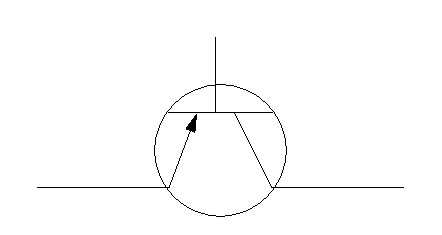
\includegraphics{./transistor.pdf}%
\end{picture}%
\setlength{\unitlength}{3947sp}%
%
\begingroup\makeatletter\ifx\SetFigFont\undefined%
\gdef\SetFigFont#1#2#3#4#5{%
  \reset@font\fontsize{#1}{#2pt}%
  \fontfamily{#3}\fontseries{#4}\fontshape{#5}%
  \selectfont}%
\fi\endgroup%
\begin{picture}(3527,1877)(1350,-2462)
\put(1501,-2161){\makebox(0,0)[lb]{\smash{{\SetFigFont{12}{14.4}{\familydefault}{\mddefault}{\updefault}{\color[rgb]{0,0,0}x}%
}}}}
\put(3076,-811){\makebox(0,0)[lb]{\smash{{\SetFigFont{12}{14.4}{\familydefault}{\mddefault}{\updefault}{\color[rgb]{0,0,0}z}%
}}}}
\put(4651,-2161){\makebox(0,0)[lb]{\smash{{\SetFigFont{12}{14.4}{\familydefault}{\mddefault}{\updefault}{\color[rgb]{0,0,0}y}%
}}}}
\end{picture}%

\end{center}
\caption{A schematic representation of a transistor.}
\label{fig:trans}
\end{figure}

Suppose that two transistors are connected as in Figure~\ref{fig:series}
(this is called a \index{series connection}{\em series} connection).  
In order for current to flow
from x to y we must have voltage applied to {\em both} the wires labeled
z and w.  In other words, this circuit effectively creates the {\bf and} 
operation --  assuming voltage is always applied to x, if z {\bf and} w
are energized then the output at y will be energized.

\begin{figure}[!hbtp] 
\begin{center}
\begin{picture}(0,0)%
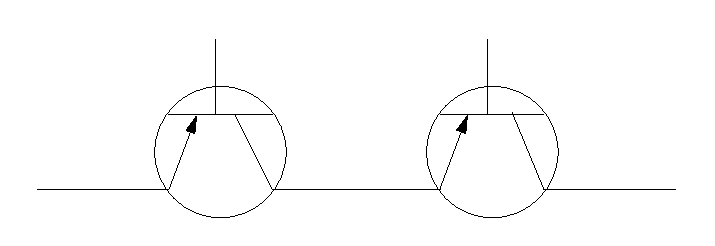
\includegraphics{figures/series.pdf}%
\end{picture}%
\setlength{\unitlength}{3947sp}%
%
\begingroup\makeatletter\ifx\SetFigFont\undefined%
\gdef\SetFigFont#1#2#3#4#5{%
  \reset@font\fontsize{#1}{#2pt}%
  \fontfamily{#3}\fontseries{#4}\fontshape{#5}%
  \selectfont}%
\fi\endgroup%
\begin{picture}(5702,1952)(1350,-2537)
\put(1501,-2161){\makebox(0,0)[lb]{\smash{{\SetFigFont{12}{14.4}{\familydefault}{\mddefault}{\updefault}{\color[rgb]{0,0,0}x}%
}}}}
\put(3076,-811){\makebox(0,0)[lb]{\smash{{\SetFigFont{12}{14.4}{\familydefault}{\mddefault}{\updefault}{\color[rgb]{0,0,0}z}%
}}}}
\put(5251,-811){\makebox(0,0)[lb]{\smash{{\SetFigFont{12}{14.4}{\familydefault}{\mddefault}{\updefault}{\color[rgb]{0,0,0}w}%
}}}}
\put(6826,-2161){\makebox(0,0)[lb]{\smash{{\SetFigFont{12}{14.4}{\familydefault}{\mddefault}{\updefault}{\color[rgb]{0,0,0}y}%
}}}}
\end{picture}%

%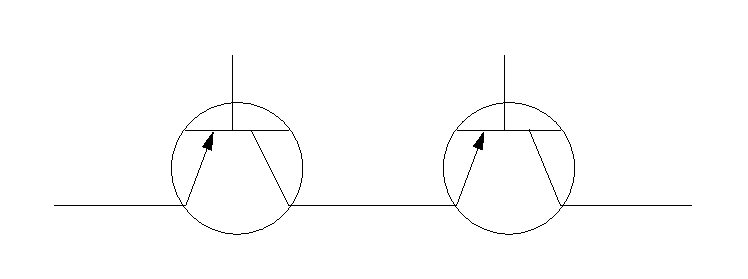
\includegraphics{series.eps}
\end{center}
\caption[Series connections implement \emph{and}.]{%
The connection of two transistors in series provides %
an implementation of the {\em and} operator.}
\label{fig:series}
\end{figure}

When two transistors are connected in \index{parallel connection}parallel (this is illustrated in
Figure~\ref{fig:par}) current can flow from x to y when either (or {\em both})
of the wires at z and w have voltage applied.  This brings up a point
which is confusing for some: in common speech the use of the word ``or'' often
has the sense known as \index{exclusive or}{\em exclusive or} (a.k.a. xor), when we say ``X or Y''
we mean ``Either X or Y, but not both.''  In Electronics and Mathematics,
{\em or} always has the non-exclusive (better known as 
\index{inclusive or}inclusive) sense.

\begin{figure}[!hbtp] 
\begin{center}
\begin{picture}(0,0)%
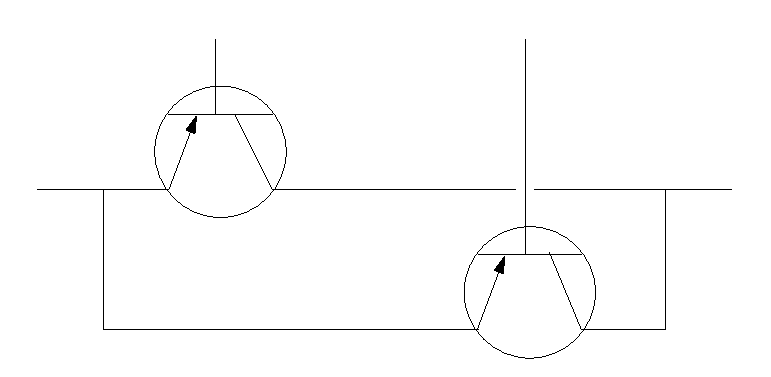
\includegraphics{./parallel.pdf}%
\end{picture}%
\setlength{\unitlength}{3947sp}%
%
\begingroup\makeatletter\ifx\SetFigFont\undefined%
\gdef\SetFigFont#1#2#3#4#5{%
  \reset@font\fontsize{#1}{#2pt}%
  \fontfamily{#3}\fontseries{#4}\fontshape{#5}%
  \selectfont}%
\fi\endgroup%
\begin{picture}(6152,3002)(1350,-3587)
\put(1501,-2161){\makebox(0,0)[lb]{\smash{{\SetFigFont{12}{14.4}{\familydefault}{\mddefault}{\updefault}{\color[rgb]{0,0,0}x}%
}}}}
\put(3076,-811){\makebox(0,0)[lb]{\smash{{\SetFigFont{12}{14.4}{\familydefault}{\mddefault}{\updefault}{\color[rgb]{0,0,0}z}%
}}}}
\put(5551,-811){\makebox(0,0)[lb]{\smash{{\SetFigFont{12}{14.4}{\familydefault}{\mddefault}{\updefault}{\color[rgb]{0,0,0}w}%
}}}}
\put(7276,-2161){\makebox(0,0)[lb]{\smash{{\SetFigFont{12}{14.4}{\familydefault}{\mddefault}{\updefault}{\color[rgb]{0,0,0}y}%
}}}}
\end{picture}%

\end{center}
\caption[Parallel connections implement \emph{or}.]{%
The connection of two transistors in parallel provides %
an implementation of the {\em or} operator.}
\label{fig:par}
\end{figure}

\newpage

As a sort of \index{logic gates}graphical shorthand, electronics engineers use the symbols
below to indicate \index{and gates}and-gates, \index{or gates}or-gates \& \index{not gates}not-gates (better known as negators).

\begin{center}
\begin{picture}(0,0)%
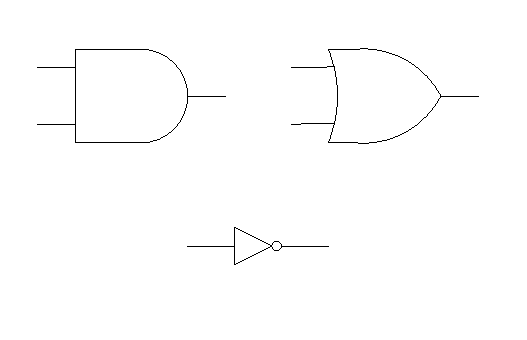
\includegraphics{figures/gates.pdf}%
\end{picture}%
\setlength{\unitlength}{3947sp}%
%
\begingroup\makeatletter\ifx\SetFigFont\undefined%
\gdef\SetFigFont#1#2#3#4#5{%
  \reset@font\fontsize{#1}{#2pt}%
  \fontfamily{#3}\fontseries{#4}\fontshape{#5}%
  \selectfont}%
\fi\endgroup%
\begin{picture}(4202,2702)(300,-2162)
\put(2026,-1861){\makebox(0,0)[lb]{\smash{{\SetFigFont{12}{14.4}{\familydefault}{\mddefault}{\updefault}{\color[rgb]{0,0,0}Not ($\lnot$)}%
}}}}
\put(2926,-961){\makebox(0,0)[lb]{\smash{{\SetFigFont{12}{14.4}{\familydefault}{\mddefault}{\updefault}{\color[rgb]{0,0,0}Or ($\lor$)}%
}}}}
\put(901,-961){\makebox(0,0)[lb]{\smash{{\SetFigFont{12}{14.4}{\familydefault}{\mddefault}{\updefault}{\color[rgb]{0,0,0}And ($\land$)}%
}}}}
\end{picture}%

\end{center}

An and-gate has two transistors inside it that are wired in series -- 
if both the inputs are energized the output will be too.  An
or-gate has two transistors in parallel inside it.  Not-gates 
involve magic -- when their input is not on, their output \emph{is}
and vice versa.

Using this graphical ``language'' one can make schematic 
representations of logical expressions.  Some find that 
tracing such diagrams makes understanding the structure 
of a Boolean expression easier.  For example, in Figure~\ref{fig:3ands}
we illustrate 2 of the possible ways that the conjunction
of four predicate variables can be parenthesized.  In fact, when
a multitude of predicates are joined by the same connective,
the way in which the expression is parenthesized is unimportant,
thus one often sees a further shorthand --- gates with more than
2 inputs.

\begin{figure}[!hbtp] 
\centerline{\begin{picture}(0,0)%
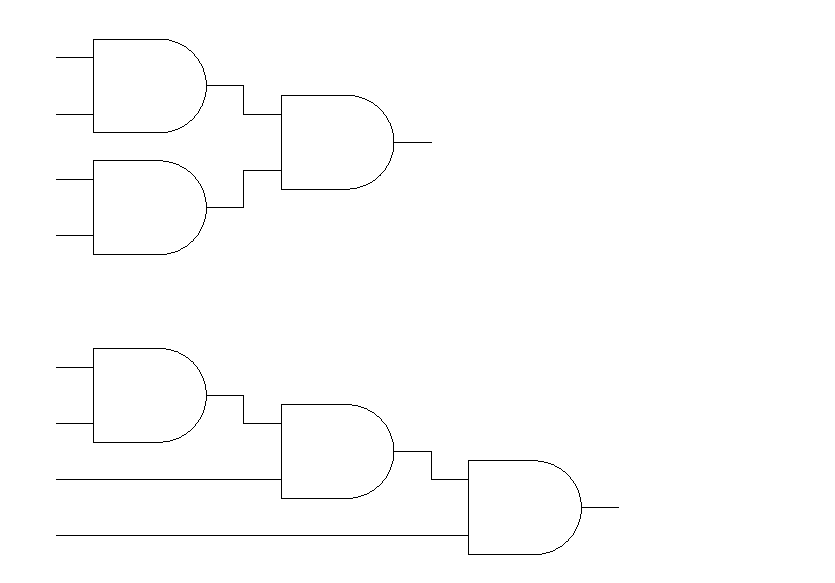
\includegraphics{figures/3_ands.pdf}%
\end{picture}%
\setlength{\unitlength}{3947sp}%
%
\begingroup\makeatletter\ifx\SetFigFont\undefined%
\gdef\SetFigFont#1#2#3#4#5{%
  \reset@font\fontsize{#1}{#2pt}%
  \fontfamily{#3}\fontseries{#4}\fontshape{#5}%
  \selectfont}%
\fi\endgroup%
\begin{picture}(6677,4652)(600,-4412)
\put(4126,-961){\makebox(0,0)[lb]{\smash{{\SetFigFont{12}{14.4}{\familydefault}{\mddefault}{\updefault}{\color[rgb]{0,0,0}$((A \land B) \land (C \land D))$}%
}}}}
\put(5626,-3886){\makebox(0,0)[lb]{\smash{{\SetFigFont{12}{14.4}{\familydefault}{\mddefault}{\updefault}{\color[rgb]{0,0,0}$(((A \land B) \land C) \land D)$}%
}}}}
\put(826,-286){\makebox(0,0)[lb]{\smash{{\SetFigFont{12}{14.4}{\familydefault}{\mddefault}{\updefault}{\color[rgb]{0,0,0}$A$}%
}}}}
\put(826,-736){\makebox(0,0)[lb]{\smash{{\SetFigFont{12}{14.4}{\familydefault}{\mddefault}{\updefault}{\color[rgb]{0,0,0}$B$}%
}}}}
\put(826,-1261){\makebox(0,0)[lb]{\smash{{\SetFigFont{12}{14.4}{\familydefault}{\mddefault}{\updefault}{\color[rgb]{0,0,0}$C$}%
}}}}
\put(826,-1711){\makebox(0,0)[lb]{\smash{{\SetFigFont{12}{14.4}{\familydefault}{\mddefault}{\updefault}{\color[rgb]{0,0,0}$D$}%
}}}}
\put(826,-2761){\makebox(0,0)[lb]{\smash{{\SetFigFont{12}{14.4}{\familydefault}{\mddefault}{\updefault}{\color[rgb]{0,0,0}$A$}%
}}}}
\put(826,-3211){\makebox(0,0)[lb]{\smash{{\SetFigFont{12}{14.4}{\familydefault}{\mddefault}{\updefault}{\color[rgb]{0,0,0}$B$}%
}}}}
\put(826,-3661){\makebox(0,0)[lb]{\smash{{\SetFigFont{12}{14.4}{\familydefault}{\mddefault}{\updefault}{\color[rgb]{0,0,0}$C$}%
}}}}
\put(826,-4111){\makebox(0,0)[lb]{\smash{{\SetFigFont{12}{14.4}{\familydefault}{\mddefault}{\updefault}{\color[rgb]{0,0,0}$D$}%
}}}}
\end{picture}%
}
\caption[Parenthesizations expressed as digital logic circuits.]{%
Two of the possible ways to parenthesize the conjunction %
of four statement variables -- expressed as digital logic circuits.}
\label{fig:3ands}
\end{figure}

A common task for an electronics designer is to come up with
a digital logic circuit having a prescribed input/output table.
Note that an input/output table for a logic circuit is entirely
analogous with a truth table for a compound sentence in Logic ---
except that we use 0's and 1's rather than T's and $\phi$'s.

Suppose that we wanted to design a circuit that would
have the following input/output table.

\begin{center}
\begin{tabular}{c|c|c|c}
$\; x \;$ & $\; y \;$ & $\; z \;$ & \rule{5pt}{0pt} out \rule{5pt}{0pt} \\ \hline
0 & 0 & 0 & 0 \\
0 & 0 & 1 & 0 \\
0 & 1 & 0 & 0 \\
0 & 1 & 1 & 1 \\ \hline
1 & 0 & 0 & 0 \\ 
1 & 0 & 1 & 0 \\ 
1 & 1 & 0 & 1 \\ 
1 & 1 & 1 & 1 \\
\end{tabular}
\end{center}

A systematic method for accomplishing such a design task involves
a notion called \index{disjunctive normal form}{\em disjunctive normal form}.  
A Boolean expression
is in disjunctive normal form if it consists of the disjunction of 
one or more statements, each of which consists entirely of conjunctions
of predicate variables and/or their negations.  In other words, the {\em or}
of a bunch of {\em ands}.  In terms of digital logic circuits, the {\em and}s 
we're talking about are called \index{recognizers}{\em recognizers}.  
For example,
the following 3-input and-gates recognize the input states in
the 4th, 7th and 8th rows of the i/o table above. (These are the rows 
where the output is supposed to be 1.)

\begin{center}
\begin{picture}(0,0)%
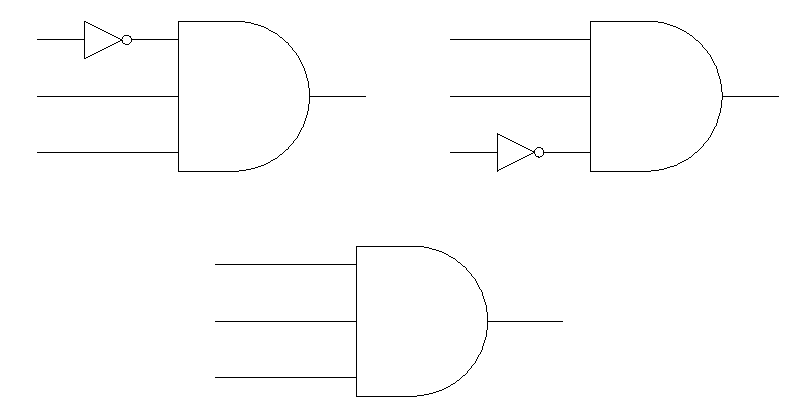
\includegraphics{./recognizers.pdf}%
\end{picture}%
\setlength{\unitlength}{3947sp}%
%
\begingroup\makeatletter\ifx\SetFigFont\undefined%
\gdef\SetFigFont#1#2#3#4#5{%
  \reset@font\fontsize{#1}{#2pt}%
  \fontfamily{#3}\fontseries{#4}\fontshape{#5}%
  \selectfont}%
\fi\endgroup%
\begin{picture}(6302,3302)(1200,-3512)
\put(1351,-586){\makebox(0,0)[lb]{\smash{{\SetFigFont{12}{14.4}{\familydefault}{\mddefault}{\updefault}{\color[rgb]{0,0,0}x}%
}}}}
\put(1351,-1036){\makebox(0,0)[lb]{\smash{{\SetFigFont{12}{14.4}{\familydefault}{\mddefault}{\updefault}{\color[rgb]{0,0,0}y}%
}}}}
\put(1351,-1486){\makebox(0,0)[lb]{\smash{{\SetFigFont{12}{14.4}{\familydefault}{\mddefault}{\updefault}{\color[rgb]{0,0,0}z}%
}}}}
\put(4651,-586){\makebox(0,0)[lb]{\smash{{\SetFigFont{12}{14.4}{\familydefault}{\mddefault}{\updefault}{\color[rgb]{0,0,0}x}%
}}}}
\put(4651,-1036){\makebox(0,0)[lb]{\smash{{\SetFigFont{12}{14.4}{\familydefault}{\mddefault}{\updefault}{\color[rgb]{0,0,0}y}%
}}}}
\put(4651,-1486){\makebox(0,0)[lb]{\smash{{\SetFigFont{12}{14.4}{\familydefault}{\mddefault}{\updefault}{\color[rgb]{0,0,0}z}%
}}}}
\put(2776,-2386){\makebox(0,0)[lb]{\smash{{\SetFigFont{12}{14.4}{\familydefault}{\mddefault}{\updefault}{\color[rgb]{0,0,0}x}%
}}}}
\put(2776,-2836){\makebox(0,0)[lb]{\smash{{\SetFigFont{12}{14.4}{\familydefault}{\mddefault}{\updefault}{\color[rgb]{0,0,0}y}%
}}}}
\put(2776,-3286){\makebox(0,0)[lb]{\smash{{\SetFigFont{12}{14.4}{\familydefault}{\mddefault}{\updefault}{\color[rgb]{0,0,0}z}%
}}}}
\end{picture}%

\end{center}

In Figure~\ref{fig:dnf} we illustrate how to create a circuit whose
i/o table is as above using these recognizers.

\begin{figure}[!hbtp] 
\begin{center}
\begin{picture}(0,0)%
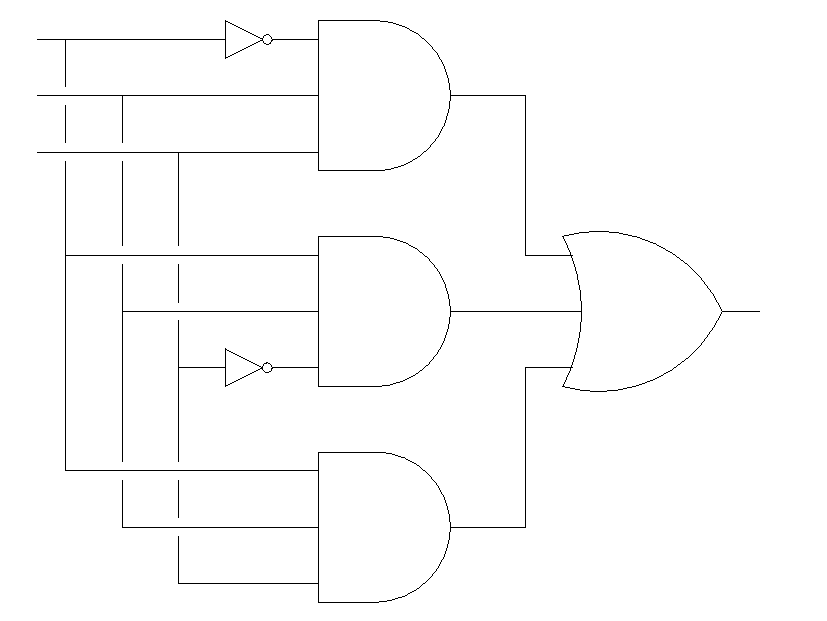
\includegraphics{./logic_circuit.pdf}%
\end{picture}%
\setlength{\unitlength}{3947sp}%
%
\begingroup\makeatletter\ifx\SetFigFont\undefined%
\gdef\SetFigFont#1#2#3#4#5{%
  \reset@font\fontsize{#1}{#2pt}%
  \fontfamily{#3}\fontseries{#4}\fontshape{#5}%
  \selectfont}%
\fi\endgroup%
\begin{picture}(6602,4952)(975,-5237)
\put(1126,-661){\makebox(0,0)[lb]{\smash{{\SetFigFont{12}{14.4}{\familydefault}{\mddefault}{\updefault}{\color[rgb]{0,0,0}x}%
}}}}
\put(1126,-1111){\makebox(0,0)[lb]{\smash{{\SetFigFont{12}{14.4}{\familydefault}{\mddefault}{\updefault}{\color[rgb]{0,0,0}y}%
}}}}
\put(1126,-1561){\makebox(0,0)[lb]{\smash{{\SetFigFont{12}{14.4}{\familydefault}{\mddefault}{\updefault}{\color[rgb]{0,0,0}z}%
}}}}
\put(7126,-2836){\makebox(0,0)[lb]{\smash{{\SetFigFont{12}{14.4}{\familydefault}{\mddefault}{\updefault}{\color[rgb]{0,0,0}out}%
}}}}
\end{picture}%

\end{center}
\caption[Disjunctive normal form.]{A digital logic circuit built % 
using disjunctive normal form.  The output of this circuit is %
$({\lnot}x \land y \land z) \lor (x \land y \land {\lnot}z) \lor (x \land y \land z)$.}
\label{fig:dnf}
\end{figure}

\newpage

\noindent{\large \bf Exercises --- \thesection\ }

\begin{enumerate}

\item Design a digital logic circuit (using and, or \& not gates) that 
implements an exclusive or.

\vspace{2in}

\item Consider the sentence 
``This is a sentence which does not refer to itself.''
which was given in the beginning of this chapter as an example.
Is this sentence a statement?  If so, what is its truth value?

\vspace{.5in}

\item Consider the sentence ``This sentence is false.''  Is this 
sentence a statement?

\vspace{.5in}

\item Complete truth tables for each of the sentences 
$(A \land B) \lor C$ and
$A \land (B \lor C)$.  Does it seem that these sentences have
the same logical content?

\vfill

\newpage

\item \label{ex:nand_nor} There are two other logical connectives that are
used somewhat less commonly than $\lor$ and $\land$.
These are the \index{Scheffer stroke} Scheffer stroke and the 
\index{Peirce arrow}Peirce arrow
-- written $\vert$ and $\downarrow$, respectively ---  they are 
also known as \index{NAND} NAND and \index{NOR} NOR.

\noindent The truth tables for these connectives are:
\medskip

\begin{tabular}{c|c|c}
$A$ & $B$ & $A \,\vert\, B$ \\ \hline
T & T & $\phi$ \\
T & $\phi$ & T \\
$\phi$ & T & T \\
$\phi$ & $\phi$ & T 
\end{tabular}
\hspace{.25 in} and \hspace{.25 in}
\begin{tabular}{c|c|c}
$A$ & $B$ & $A \downarrow B$ \\ \hline
T & T & $\phi$ \\
T & $\phi$ & $\phi$ \\
$\phi$ & T & $\phi$ \\
$\phi$ & $\phi$ & T 
\end{tabular}
\medskip

Find an expression for $(A\, \land \lnot B) \lor C$
using only these new connectives (as well as negation and the
variable symbols themselves).

\item \label{IKK} The famous logician \index{Smullyan, Raymond} Raymond Smullyan devised 
a family of logical puzzles around a fictitious place he called 
\index{Knights and Knaves} ``the Island of Knights and Knaves.''  The inhabitants of the island are either knaves, who always make false statements, or knights, who always make truthful statements.  

In the most famous knight/knave puzzle, you are in a room which has only two exits.  One leads to certain death and the other to freedom.  There are two 
individuals in the room, and you know that one of them is a knight and the other is a knave, but you don't know which.   Your challenge is to determine the door which leads to freedom by asking a single question.

\end{enumerate}


\newpage

\section{Implication}
\label{sec:impl}

Suppose a mother makes the following statement to her child:
``If you finish your peas, you'll get dessert.''

This is a compound sentence made up of the two simpler
sentences $P=$ ``You finish your peas'' and $D=$ ``You'll get dessert.''
It is an example of a type of compound sentence called a 
\index{conditional statement}{\em conditional}.  Conditionals are if-then type statements.  
In ordinary language the word ``then'' is often elided (as is the case
with our example above).  Another way of phrasing the ``If P then D.'' 
relationship is to use the word ``implies'' --- although it would be
a rather uncommon mother who would say ``Finishing your peas implies
that you will receive dessert.'' 

As was the case in the previous section, there are four possible
situations and we must consider each to decide the truth/falsity 
of this conditional statement.  The peas may or may not be finished,
and independently, the dessert may or may not be proffered.   

Suppose the child finishes the peas and the mother comes across
with the dessert.  Clearly, in this situation the mother's statement 
was true.  On the other hand, if the child finishes the hated peas
and yet does not receive a treat, it is just as obvious that the 
mother has lied! 
What do we say about the mother's veracity in the case that the peas
go unfinished?  Here, Mom gets a break.  She can either hold firm
and deliver no dessert, or she can be a softy and give out unearned 
sweets -- in either case, we can't accuse her of telling a falsehood.
The statement she made had to do {\em only} with the eventualities
following total pea consumption, she said nothing about what happens
if the peas go uneaten.

A conditional statement's components are called the 
\index{antecedent}{\em antecedent} 
(this is the ``if'' part, as in ``finish
your peas'') and the \index{consequent}{\em consequent} (this is the ``then'' part, as in
``get dessert'').  The discussion in the 
last paragraph was intended to make the point that when the antecedent
is false, we should consider the conditional to be true.  Conditionals
that are true because their antecedents are false are said to
be \index{vacuous truth}{\em vacuously true}.  The conditional 
involving an antecedent $A$
and a consequent $B$ is expressed symbolically using an arrow: 
$A \implies B$.  Here is a truth table for this connective.

\begin{center}
\begin{tabular}{c|c||c}
\; $A$ \; & \; $B$ \; & \; $A \implies B$ \; \\ \hline
T & T & T \\
T & $\phi$ & $\phi$\\
 $\phi$ & T & T \\
 $\phi$ &  $\phi$ & T\\
\end{tabular}
\end{center}

\begin{exer} 
Note that this truth table is similar to the truth table for
$A \lor B$ in that there is only a single row having a $\phi$ in
the last column.  For $A \lor B$ the $\phi$ occurs in the 4th row
and for $A \implies B$ it occurs in the 2nd row.  This suggests
that by suitably modifying things (replacing $A$ or $B$ by their
negations) we could come up with an ``or'' statement that had the 
same meaning as the conditional.  Try it!
\end{exer}

It is fairly common that conditionals are used to express threats,
as in the peas/dessert example.  Another common way to express a 
threat is to use a disjunction -- ``Finish your peas, or you won't
get dessert.''  If you've been paying attention (and did the last
exercise), you will notice that this is {\em  not} the disjunction
that should have the same meaning as the original conditional.  
There is probably no mother on Earth who would say
``Don't finish your peas, or you get dessert!'' to her child
(certainly not if she expects to be understood).  So what's going on
here?

The problem is that ``Finish your peas, or you won't
get dessert.'' has the same logical content as
``If you get dessert then you finished your peas.''
(Notice that the roles of the antecedent and consequent have been
switched.)  And, while this last sentence sounds awkward, it is
probably a more accurate reflection of what the mother intended.
The problem {\em really} is that people are incredibly sloppy 
with their conditional statements!  A lot of people secretly want 
the 3rd row of the truth table for $\implies$ to have a $\phi$
in it, and it simply doesn't!  The operator that results if we do
make this modification is called the \index{biconditional}
biconditional, and is expressed
in English using the phrase ``if and only if'' (which leads mathematicians
to the abbreviation \index{iff}``iff'' much to the consternation of 
spell-checking programs everywhere).  The biconditional is denoted 
using an arrow that points both ways.  Its truth table follows.

\begin{center}
\begin{tabular}{c|c||c}
\; $A$ \; & \; $B$ \; & \; $A \iff B$ \; \\ \hline
T & T & T \\
T & $\phi$ & $\phi$\\
 $\phi$ & T & $\phi$ \\
 $\phi$ &  $\phi$ & T\\
\end{tabular}
\end{center}

Please note, that while we like to strive for precision, we do not
necessarily recommend the use of phrases such as 
``You will receive dessert if, and only if,
you finish your peas.'' with young children.


Since conditional sentences are often confused with the sentence
that has the roles of antecedent and consequent reversed, this
switched-around sentence has been given a name: it is the 
\index{converse}{\em converse}
of the original statement.  Another conditional that is distinct from 
(but related to) a given conditional is its \index{inverse}{\em inverse}.  
This sort of sentence probably had to be named because of a very common 
misconception, many people think that the way to negate an if-then 
proposition is to negate
its parts.  Algebraically, this looks reasonable -- sort of a distributive
law for logical negation over implications -- $\lnot( A \implies B) =
{\lnot}A \implies {\lnot}B$.  Sadly, this reasonable looking assertion
can't possibly be true; since implications have just one $\phi$ in a truth 
table, the negation of an implication  must have three -- but the statement 
with the $\lnot$'s on the {\em parts} of the implication is going to only have 
a single $\phi$ in {\em its} truth table.

To recap, the converse of an implication has the pieces (antecedent and 
consequent) switched about.  The inverse of an implication has the 
pieces negated.  Neither of these is the same as the original implication.
Oddly, this is one of those times when two wrongs {\em do} make a right.
If you start with an implication, form its converse, then take the inverse
of that, you get a statement having exactly the same logical meaning
as the original.  This new statement is called the 
\index{contrapositive}{\em contrapositive}.

This information is displayed in Table~\ref{tab:contra} 

\begin{table}[hbt] 
\begin{center}
\begin{tabular}{cc} 
 & converses \\
 & %
\ifx\pdfoutput\undefined % We're not running pdftex
 
\includegraphics{figures/horiz_arrows.eps} \\%
\else
 
\includegraphics{figures/horiz_arrows.pdf} \\%
\fi
\parbox[c]{10pt}{ \begin{sideways} inverses \end{sideways} } 
\parbox[c]{10pt}{ 
\ifx\pdfoutput\undefined % We're not running pdftex
 
\includegraphics{figures/vert_arrows.eps}% 
\else

\includegraphics{figures/vert_arrows.pdf}% 
\fi } & %
\begin{tabular}{|ccc|ccc|} \hline
 \rule{20pt}{0pt} & \rule{0pt}{20pt} & \rule{20pt}{0pt} & \rule{20pt}{0pt} & \rule{0pt}{20pt} & \rule{20pt}{0pt} \\
 & $A \implies B$ & & & $B \implies A$ & \\
 \rule{0pt}{20pt} & & & & & \\ \hline
 \rule{0pt}{20pt} & & & & & \\
 & ${\lnot}A \implies {\lnot}B$ & & & ${\lnot}B \implies {\lnot}A$ & \\ 
\rule{0pt}{20pt} & & & & & \\ \hline
\end{tabular} \\
\end{tabular}
\end{center}
\caption[Converse, inverse and contrapositive.]{The relationship %
between a conditional statement, its converse, its inverse and its %
contrapositive.}
\label{tab:contra}
\end{table}


One final piece of advice about conditionals: don't confuse logical
if-then relationships with causality.  Many of the if-then sentences
we run into in ordinary life describe cause and effect:  
``If you cut the green wire the bomb will explode.''  (Okay, that one
is an example from the ordinary life of a bomb squad technician, but \ldots)
It is usually best to think of the if-then relationships we find in
Logic as divorced from the flow of time, the fact that $A \implies B$
is logically the same as ${\lnot}A \lor B$ lends credence to this point of view.

\newpage

\noindent{\large \bf Exercises --- \thesection\ }

\begin{enumerate}

\item The transitive property of equality says that if $a=b$ and $b=c$
then $a=c$.  Does the implication arrow satisfy a transitive property?
If so, state it.

\item Complete truth tables for the compound sentences $A \implies B$ and
  ${\lnot}A \lor B$.

\item Complete a truth table for the compound sentence $A \implies (B \implies C)$ and for the sentence $(A \implies B) \implies C$.  What can you conclude
about conditionals and the associative property?

\item Determine a sentence using the {\em and} connector ($\land$) that
gives the negation of $A \implies B$.

\item Rewrite the sentence ``Fix the toilet or I won't pay the rent!'' as
a conditional.

\item Why is it that the sentence ``If pigs can fly, I am the king
of Mesopotamia.'' true?

\item Express the statement $A \implies B$ using the Peirce arrow and/or the
Scheffer stroke. (See Exercise~\ref{ex:nand_nor} in the previous section.)

\item Find the contrapositives of the following sentences.
  \begin{enumerate}
  \item If you can't do the time, don't do the crime.
  \item If you do well in school, you'll get a good job.
  \item If you wish others to treat you in a certain way, you must 
    treat others in that fashion.
  \item If it's raining, there must be clouds.
  \item If $a_n \leq b_n$, for all $n$ and $\sum_{n=0}^\infty b_n$ is a 
convergent series, then $\sum_{n=0}^\infty a_n$ is a convergent series.
  \end{enumerate}

\item What are the converse and inverse of ``If you watch my back, I'll 
watch your back.''?

\item The integral test in Calculus is used to determine whether an
infinite series converges or diverges:   Suppose that $f(x)$ is a positive,
decreasing, 
real-valued function with $\lim_{x \longrightarrow \infty} f(x) = 0$, if
the improper integral
$\int_0^\infty f(x)$ has a finite value, then the infinite series 
$\sum_{n=1}^\infty f(n)$ converges.

The integral test should be envisioned by letting the series correspond
to a right-hand Riemann sum for the integral, since the function is decreasing,
a right-hand Riemann sum is an underestimate for the value of the integral,
thus

\[ \sum_{n=1}^\infty f(n) < \int_0^\infty f(x). \]

Discuss the meanings of and (where possible) provide justifications for
the inverse, converse and contrapositive of the conditional statement 
in the integral test.

\item On the Island of Knights and Knaves (see page~\pageref{IKK}) you encounter two individuals named Locke and Demosthenes.  

Locke says, ``Demosthenes is a knave.'' \newline
Demosthenes says ``Locke and I are knights.''

Who is a knight and who a knave?

\end{enumerate}


\newpage

\section{Logical equivalences}
\label{sec:le}

Some logical statements are ``the same.''  For example, in the last
section, we discussed the fact that a conditional
and its contrapositive have the same logical content.  Wouldn't
we be justified in writing something like the following?

\[ A \implies B \; = \; {\lnot}B \implies {\lnot}A \]

Well, one pretty serious objection to doing that is that the 
equals sign ($=$) has already got a job; it is used to indicate that
two numerical quantities are the same.  What we're doing here is 
really sort of a different thing!  Nevertheless, there is a concept
of ``sameness'' between certain compound statements, and we need a 
symbolic way of expressing it.  There are two notations in common 
use.  The notation that seems to be preferred by logicians is the
biconditional ($\iff$).  The notation we'll use
in the rest of this book is an equals sign with a bit of extra decoration
on it ($\cong$).  

Thus we can can either write 

\[ (A \implies B) \; \iff \; ({\lnot}B \implies {\lnot}A) \]

\noindent or 

\[ A \implies B \; \cong \; {\lnot}B \implies {\lnot}A. \]

\noindent I like the latter, but use whichever form you like -- no one
will have any problem understanding either.

The formal definition of \index{logical equivalence}{\em logical equivalence}, 
which is what we've
been describing, is this:  two compound sentences are logically equivalent
if in a truth table (that contains all possible combinations of the 
truth values of the predicate variables in its rows) the truth values
of the two sentences are equal in every row. 

\begin{exer} 
Consider the two compound sentences $A \lor B$ and $A \lor ({\lnot}A \land B)$.
There are a total of 2 predicate variables between them, so a truth table
with 4 rows will suffice.  Fill out the missing entries in the truth
table and determine whether the statements are equivalent.

\begin{center}
\begin{tabular}{c|c||c|c}
\; $A$ \; & \; $B$ \; & \; $A \lor B$ \; & \; $A \lor ({\lnot}A \land B)$\; \\ \hline
T & T &  & \\
T & $\phi$ & & \\
 $\phi$ & T & &  \\
 $\phi$ &  $\phi$  & &\\
\end{tabular}
\end{center}

\end{exer}

One could, in principle, verify all logical equivalences by filling out
truth tables.  Indeed, in the exercises for this section we will ask you
to develop a certain facility at this task.  While this activity can
be somewhat fun, and many of my students want the filling-out of truth 
tables to
be a significant portion of their midterm exam, you will probably eventually
come to find it somewhat tedious.  A slightly more mature approach to logical
equivalences is this: use a set of basic equivalences -- which themselves
may be verified via truth tables -- as the basic {\em rules} or 
\index{laws of logical equivalence}{\em laws}
of logical equivalence, and develop a strategy for converting one
sentence into another using these rules.  This process will feel very
familiar, it is like ``doing'' algebra, but the rules one is allowed 
to use are subtly different.

First we have the \index{commutative law}{\em commutative laws}, 
one each for conjunction
and disjunction.  It's worth noting that there {\em isn't} a commutative
law for implication.   

The commutative property of conjunction says that $A \land B \cong B \land A$.
This is quite an apparent statement from the perspective of linguistics.
Surely it's the same thing to say ``the weather is cold and snowy'' as it is to
say ``the weather is snowy and cold.''   
This commutative property is also clear 
from the perspective of digital logic circuits.

\begin{center}
\begin{picture}(0,0)%
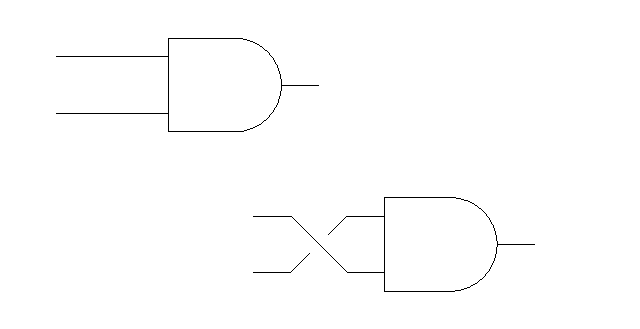
\includegraphics{./comm_conj.pdf}%
\end{picture}%
\setlength{\unitlength}{3947sp}%
%
\begingroup\makeatletter\ifx\SetFigFont\undefined%
\gdef\SetFigFont#1#2#3#4#5{%
  \reset@font\fontsize{#1}{#2pt}%
  \fontfamily{#3}\fontseries{#4}\fontshape{#5}%
  \selectfont}%
\fi\endgroup%
\begin{picture}(5102,2627)(1125,-2987)
\put(2926,-2611){\makebox(0,0)[lb]{\smash{{\SetFigFont{12}{14.4}{\familydefault}{\mddefault}{\updefault}{\color[rgb]{0,0,0}$B$}%
}}}}
\put(2926,-2161){\makebox(0,0)[lb]{\smash{{\SetFigFont{12}{14.4}{\familydefault}{\mddefault}{\updefault}{\color[rgb]{0,0,0}$A$}%
}}}}
\put(5476,-2386){\makebox(0,0)[lb]{\smash{{\SetFigFont{12}{14.4}{\familydefault}{\mddefault}{\updefault}{\color[rgb]{0,0,0}$B \land A$}%
}}}}
\put(3751,-1111){\makebox(0,0)[lb]{\smash{{\SetFigFont{12}{14.4}{\familydefault}{\mddefault}{\updefault}{\color[rgb]{0,0,0}$A \land B$}%
}}}}
\put(1351,-1336){\makebox(0,0)[lb]{\smash{{\SetFigFont{12}{14.4}{\familydefault}{\mddefault}{\updefault}{\color[rgb]{0,0,0}$B$}%
}}}}
\put(1351,-886){\makebox(0,0)[lb]{\smash{{\SetFigFont{12}{14.4}{\familydefault}{\mddefault}{\updefault}{\color[rgb]{0,0,0}$A$}%
}}}}
\end{picture}%

\end{center}   
  
The commutative property of disjunctions is equally transparent from
the perspective of a circuit diagram.  

\begin{center}
\begin{picture}(0,0)%
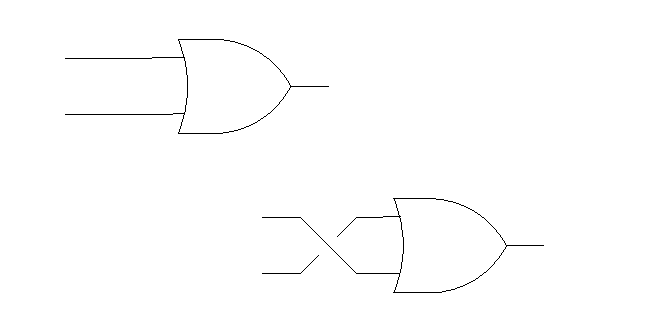
\includegraphics{figures/comm_disj.pdf}%
\end{picture}%
\setlength{\unitlength}{3947sp}%
%
\begingroup\makeatletter\ifx\SetFigFont\undefined%
\gdef\SetFigFont#1#2#3#4#5{%
  \reset@font\fontsize{#1}{#2pt}%
  \fontfamily{#3}\fontseries{#4}\fontshape{#5}%
  \selectfont}%
\fi\endgroup%
\begin{picture}(5177,2552)(1050,-2912)
\put(2926,-2611){\makebox(0,0)[lb]{\smash{{\SetFigFont{12}{14.4}{\familydefault}{\mddefault}{\updefault}{\color[rgb]{0,0,0}$B$}%
}}}}
\put(2926,-2161){\makebox(0,0)[lb]{\smash{{\SetFigFont{12}{14.4}{\familydefault}{\mddefault}{\updefault}{\color[rgb]{0,0,0}$A$}%
}}}}
\put(1351,-1336){\makebox(0,0)[lb]{\smash{{\SetFigFont{12}{14.4}{\familydefault}{\mddefault}{\updefault}{\color[rgb]{0,0,0}$B$}%
}}}}
\put(1351,-886){\makebox(0,0)[lb]{\smash{{\SetFigFont{12}{14.4}{\familydefault}{\mddefault}{\updefault}{\color[rgb]{0,0,0}$A$}%
}}}}
\put(3751,-1111){\makebox(0,0)[lb]{\smash{{\SetFigFont{12}{14.4}{\familydefault}{\mddefault}{\updefault}{\color[rgb]{0,0,0}$A \lor B$}%
}}}}
\put(5476,-2386){\makebox(0,0)[lb]{\smash{{\SetFigFont{12}{14.4}{\familydefault}{\mddefault}{\updefault}{\color[rgb]{0,0,0}$B \lor A$}%
}}}}
\end{picture}%

\end{center}   
  
The \index{associative law}{\em associative laws} also have something to do with what order operations
are done.  One could think of the difference in the following terms:  
Commutative properties
involve spatial or physical order and the associative properties involve
temporal order.  The associative law of addition could be used to say we'll
get the same result if we add 2 and 3 first, then add 4, or if we add 2 to the 
sum of 3 and 4 (i.e. that $(2+3)+4$ is the same as $2+(3+4)$.)  Note that 
physically, the numbers are in the same order (2 then 3 then 4) in both 
expressions but that the parentheses indicate a precedence in {\em when} the
plus signs are evaluated. 

The associative law of conjunction states that $A \land (B \land C) \cong
(A \land B) \land C$.  In visual terms, this means the following two 
circuit diagrams are equivalent.

\begin{center}
\begin{picture}(0,0)%
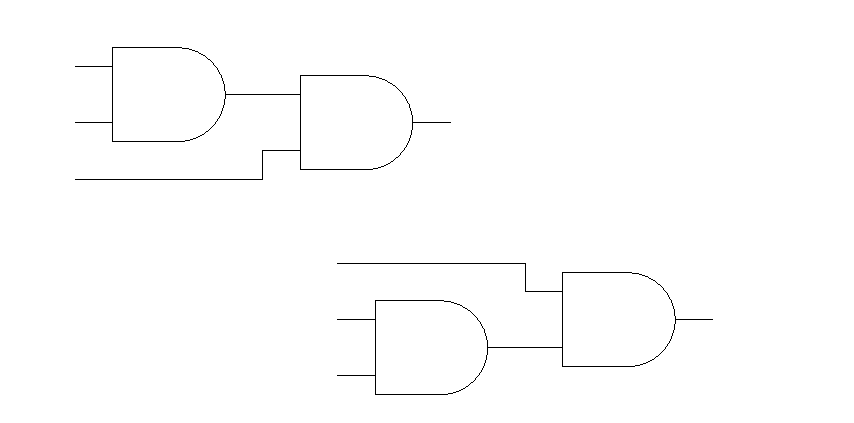
\includegraphics{./assoc_conj.pdf}%
\end{picture}%
\setlength{\unitlength}{3947sp}%
%
\begingroup\makeatletter\ifx\SetFigFont\undefined%
\gdef\SetFigFont#1#2#3#4#5{%
  \reset@font\fontsize{#1}{#2pt}%
  \fontfamily{#3}\fontseries{#4}\fontshape{#5}%
  \selectfont}%
\fi\endgroup%
\begin{picture}(6827,3377)(225,-3437)
\put(601,-661){\makebox(0,0)[lb]{\smash{{\SetFigFont{12}{14.4}{\familydefault}{\mddefault}{\updefault}{\color[rgb]{0,0,0}$A$}%
}}}}
\put(601,-1111){\makebox(0,0)[lb]{\smash{{\SetFigFont{12}{14.4}{\familydefault}{\mddefault}{\updefault}{\color[rgb]{0,0,0}$B$}%
}}}}
\put(601,-1561){\makebox(0,0)[lb]{\smash{{\SetFigFont{12}{14.4}{\familydefault}{\mddefault}{\updefault}{\color[rgb]{0,0,0}$C$}%
}}}}
\put(3901,-1111){\makebox(0,0)[lb]{\smash{{\SetFigFont{12}{14.4}{\familydefault}{\mddefault}{\updefault}{\color[rgb]{0,0,0}$(A \land B) \land C$}%
}}}}
\put(2701,-2236){\makebox(0,0)[lb]{\smash{{\SetFigFont{12}{14.4}{\familydefault}{\mddefault}{\updefault}{\color[rgb]{0,0,0}$A$}%
}}}}
\put(2701,-2686){\makebox(0,0)[lb]{\smash{{\SetFigFont{12}{14.4}{\familydefault}{\mddefault}{\updefault}{\color[rgb]{0,0,0}$B$}%
}}}}
\put(2701,-3136){\makebox(0,0)[lb]{\smash{{\SetFigFont{12}{14.4}{\familydefault}{\mddefault}{\updefault}{\color[rgb]{0,0,0}$C$}%
}}}}
\put(6001,-2686){\makebox(0,0)[lb]{\smash{{\SetFigFont{12}{14.4}{\familydefault}{\mddefault}{\updefault}{\color[rgb]{0,0,0}$A \land (B \land C)$}%
}}}}
\end{picture}%

\end{center}   
  
The associative law of disjunction states that $A \lor (B \lor C) \cong
(A \lor B) \lor C$.  Visually, this looks like:

\begin{center}
\begin{picture}(0,0)%
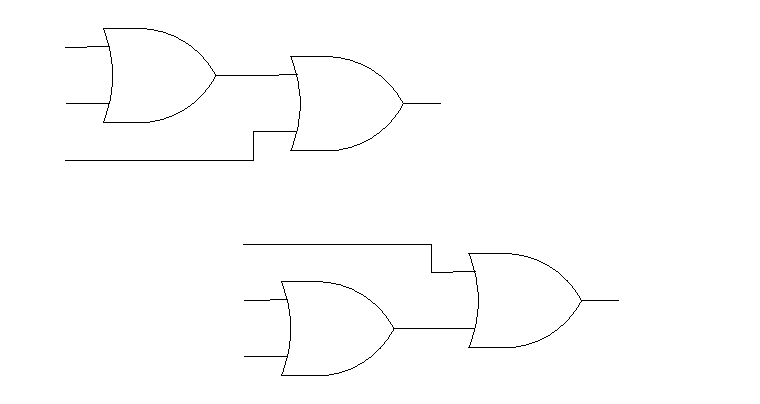
\includegraphics{./assoc_disj.pdf}%
\end{picture}%
\setlength{\unitlength}{3947sp}%
%
\begingroup\makeatletter\ifx\SetFigFont\undefined%
\gdef\SetFigFont#1#2#3#4#5{%
  \reset@font\fontsize{#1}{#2pt}%
  \fontfamily{#3}\fontseries{#4}\fontshape{#5}%
  \selectfont}%
\fi\endgroup%
\begin{picture}(6077,3227)(375,-2987)
\put(676,-211){\makebox(0,0)[lb]{\smash{{\SetFigFont{12}{14.4}{\familydefault}{\mddefault}{\updefault}{\color[rgb]{0,0,0}$A$}%
}}}}
\put(676,-661){\makebox(0,0)[lb]{\smash{{\SetFigFont{12}{14.4}{\familydefault}{\mddefault}{\updefault}{\color[rgb]{0,0,0}$B$}%
}}}}
\put(676,-1111){\makebox(0,0)[lb]{\smash{{\SetFigFont{12}{14.4}{\familydefault}{\mddefault}{\updefault}{\color[rgb]{0,0,0}$C$}%
}}}}
\put(3976,-661){\makebox(0,0)[lb]{\smash{{\SetFigFont{12}{14.4}{\familydefault}{\mddefault}{\updefault}{\color[rgb]{0,0,0}$(A \lor B) \lor C$}%
}}}}
\put(2101,-1786){\makebox(0,0)[lb]{\smash{{\SetFigFont{12}{14.4}{\familydefault}{\mddefault}{\updefault}{\color[rgb]{0,0,0}$A$}%
}}}}
\put(2101,-2236){\makebox(0,0)[lb]{\smash{{\SetFigFont{12}{14.4}{\familydefault}{\mddefault}{\updefault}{\color[rgb]{0,0,0}$B$}%
}}}}
\put(2101,-2686){\makebox(0,0)[lb]{\smash{{\SetFigFont{12}{14.4}{\familydefault}{\mddefault}{\updefault}{\color[rgb]{0,0,0}$C$}%
}}}}
\put(5401,-2236){\makebox(0,0)[lb]{\smash{{\SetFigFont{12}{14.4}{\familydefault}{\mddefault}{\updefault}{\color[rgb]{0,0,0}$A \lor (B \lor C)$}%
}}}}
\end{picture}%

\end{center}   
  

\begin{exer}
In a situation where {\em both} associativity and commutativity pertain
the symbols involved can appear in any order and with any reasonable 
parenthesization.  In how many different ways can the sum $2+3+4$ 
be expressed?  Only consider expression that are fully parenthesized.
\end{exer}
 
The next type of basic logical equivalences we'll consider are the
so-called \index{distributive law}{\em distributive laws}.  
Distributive laws involve the 
interaction of two operations, when we distribute multiplication 
over a sum, we effectively replace one instance of an operand {\em 
and the associated operator}, with two instances, as is illustrated
below.

\begin{center}
\begin{picture}(0,0)%
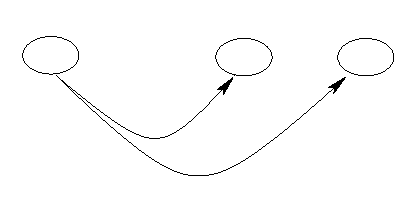
\includegraphics{./dist_2x3+4.pdf}%
\end{picture}%
\setlength{\unitlength}{3947sp}%
%
\begingroup\makeatletter\ifx\SetFigFont\undefined%
\gdef\SetFigFont#1#2#3#4#5{%
  \reset@font\fontsize{#1}{#2pt}%
  \fontfamily{#3}\fontseries{#4}\fontshape{#5}%
  \selectfont}%
\fi\endgroup%
\begin{picture}(3227,1577)(1125,-4337)
\put(1426,-3286){\makebox(0,0)[lb]{\smash{{\SetFigFont{12}{14.4}{\familydefault}{\mddefault}{\updefault}{\color[rgb]{0,0,0}2  *  ( 3 + 4 ) = ( 2  *  3 ) + ( 2  *  4 )}%
}}}}
\end{picture}%

\end{center}   
  
The logical operators $\land$ and $\lor$ each distribute over the other.
Thus we have the distributive law of conjunction over disjunction, which
is expressed in the equivalence 
$A \land (B \lor C) \cong (A \land B) \lor (A \land C)$ 
and in the following digital logic circuit diagram.

\begin{center}
\begin{picture}(0,0)%
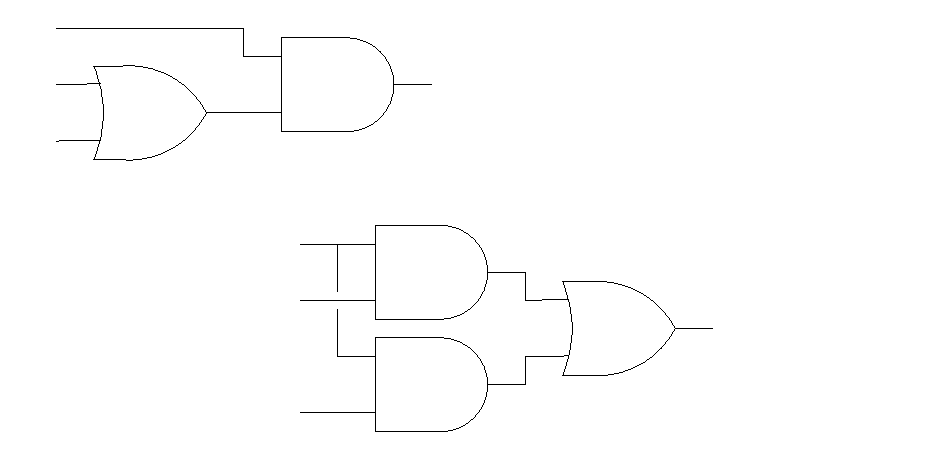
\includegraphics{./dist_and_o_or.pdf}%
\end{picture}%
\setlength{\unitlength}{3947sp}%
%
\begingroup\makeatletter\ifx\SetFigFont\undefined%
\gdef\SetFigFont#1#2#3#4#5{%
  \reset@font\fontsize{#1}{#2pt}%
  \fontfamily{#3}\fontseries{#4}\fontshape{#5}%
  \selectfont}%
\fi\endgroup%
\begin{picture}(7427,3677)(600,-3737)
\put(826,-1261){\makebox(0,0)[lb]{\smash{{\SetFigFont{12}{14.4}{\familydefault}{\mddefault}{\updefault}{\color[rgb]{0,0,0}$C$}%
}}}}
\put(826,-811){\makebox(0,0)[lb]{\smash{{\SetFigFont{12}{14.4}{\familydefault}{\mddefault}{\updefault}{\color[rgb]{0,0,0}$B$}%
}}}}
\put(826,-361){\makebox(0,0)[lb]{\smash{{\SetFigFont{12}{14.4}{\familydefault}{\mddefault}{\updefault}{\color[rgb]{0,0,0}$A$}%
}}}}
\put(4126,-811){\makebox(0,0)[lb]{\smash{{\SetFigFont{12}{14.4}{\familydefault}{\mddefault}{\updefault}{\color[rgb]{0,0,0}$A \land (B \lor C)$}%
}}}}
\put(2776,-2086){\makebox(0,0)[lb]{\smash{{\SetFigFont{12}{14.4}{\familydefault}{\mddefault}{\updefault}{\color[rgb]{0,0,0}$A$}%
}}}}
\put(2776,-2536){\makebox(0,0)[lb]{\smash{{\SetFigFont{12}{14.4}{\familydefault}{\mddefault}{\updefault}{\color[rgb]{0,0,0}$B$}%
}}}}
\put(2776,-3436){\makebox(0,0)[lb]{\smash{{\SetFigFont{12}{14.4}{\familydefault}{\mddefault}{\updefault}{\color[rgb]{0,0,0}$C$}%
}}}}
\put(6376,-2761){\makebox(0,0)[lb]{\smash{{\SetFigFont{12}{14.4}{\familydefault}{\mddefault}{\updefault}{\color[rgb]{0,0,0}$(A \land B) \lor (A \land C)$}%
}}}}
\end{picture}%

\end{center}   

We also have the distributive law of disjunction over conjunction 
which is given by the equivalence 
$A \lor (B \land C) \cong (A \lor B) \land (A \lor C)$ and in the 
circuit diagram:

\begin{center}
\begin{picture}(0,0)%
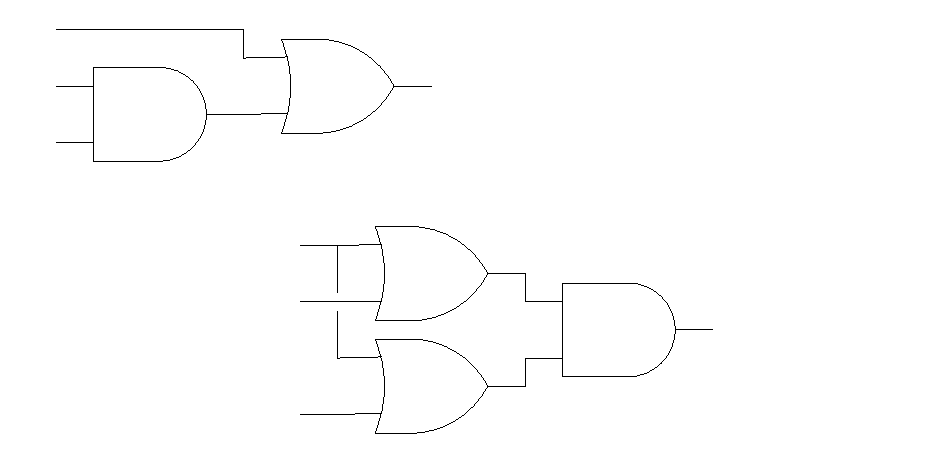
\includegraphics{./dist_or_o_and.pdf}%
\end{picture}%
\setlength{\unitlength}{3947sp}%
%
\begingroup\makeatletter\ifx\SetFigFont\undefined%
\gdef\SetFigFont#1#2#3#4#5{%
  \reset@font\fontsize{#1}{#2pt}%
  \fontfamily{#3}\fontseries{#4}\fontshape{#5}%
  \selectfont}%
\fi\endgroup%
\begin{picture}(7427,3602)(600,-3662)
\put(2776,-2086){\makebox(0,0)[lb]{\smash{{\SetFigFont{12}{14.4}{\familydefault}{\mddefault}{\updefault}{\color[rgb]{0,0,0}$A$}%
}}}}
\put(2776,-2536){\makebox(0,0)[lb]{\smash{{\SetFigFont{12}{14.4}{\familydefault}{\mddefault}{\updefault}{\color[rgb]{0,0,0}$B$}%
}}}}
\put(2776,-3436){\makebox(0,0)[lb]{\smash{{\SetFigFont{12}{14.4}{\familydefault}{\mddefault}{\updefault}{\color[rgb]{0,0,0}$C$}%
}}}}
\put(6376,-2761){\makebox(0,0)[lb]{\smash{{\SetFigFont{12}{14.4}{\familydefault}{\mddefault}{\updefault}{\color[rgb]{0,0,0}$(A \lor B) \land (A \lor C)$}%
}}}}
\put(826,-1261){\makebox(0,0)[lb]{\smash{{\SetFigFont{12}{14.4}{\familydefault}{\mddefault}{\updefault}{\color[rgb]{0,0,0}$C$}%
}}}}
\put(826,-811){\makebox(0,0)[lb]{\smash{{\SetFigFont{12}{14.4}{\familydefault}{\mddefault}{\updefault}{\color[rgb]{0,0,0}$B$}%
}}}}
\put(826,-361){\makebox(0,0)[lb]{\smash{{\SetFigFont{12}{14.4}{\familydefault}{\mddefault}{\updefault}{\color[rgb]{0,0,0}$A$}%
}}}}
\put(4126,-811){\makebox(0,0)[lb]{\smash{{\SetFigFont{12}{14.4}{\familydefault}{\mddefault}{\updefault}{\color[rgb]{0,0,0}$A \lor (B \land C)$}%
}}}}
\end{picture}%

\end{center}   

Traditionally, the laws we've just stated would be called 
{\em left}-distributive laws and we would also need to state 
that there are {\em right}-distributive laws that apply.  Since,
in the current setting, we have already said that the commutative
law is valid, this isn't really necessary.

\begin{exer}
State the right-hand versions of the distributive laws.
\end{exer}

The next set of laws we'll consider come from trying to
figure out what the distribution of a minus sign over a sum
($-(x+y) = -x + -y$)
should correspond to in Boolean algebra.  At first blush one 
might assume the analogous thing in Boolean algebra would be
something like ${\lnot}(A \land B) \cong {\lnot}A \land {\lnot}B$,
but we can easily dismiss this by looking at a truth table.

\begin{center}
\begin{tabular}{c|c||c|c}
\; $A$ \; & \; $B$ \; & \; ${\lnot}(A \land B)$ \; & \; ${\lnot}A \land {\lnot}B$\; \\ \hline
T & T &  $\phi$ & $\phi$ \\
T & $\phi$ & T & $\phi$ \\
 $\phi$ & T & T & $\phi$ \\
 $\phi$ &  $\phi$  & T & T\\
\end{tabular}
\end{center}

What actually works is a set of rules known as 
\index{DeMorgan's laws}DeMorgan's laws, which
basically say that you distribute the negative sign but
you also must change the operator.  As logical equivalences,
DeMorgan's laws are 

\[ {\lnot}(A \land B) \; \cong \; {\lnot}A \lor {\lnot}B \]

\noindent and

\[ {\lnot}(A \lor B) \; \cong \; {\lnot}A \land {\lnot}B. \]

In ordinary arithmetic there are two notions of ``inverse.''  The 
{\em negative} of a number is known as its additive inverse and
the {\em reciprocal} of a number is its multiplicative inverse.
These notions lead to a couple of equations,

\[ x + -x = 0 \]

\noindent and

\[ x \cdot \frac{1}{x} = 1. \]

\noindent Boolean algebra only has one ``inverse'' concept, the denial
 of a predicate (i.e. logical negation), but the equations above have analogues, as do
the symbols $0$ and $1$ that appear in them.  First, consider
the Boolean expression $A \lor {\lnot}A$.  This is the logical {\em or}
of a statement and its exact opposite; when one is true the other is 
false and vice versa.  But, the disjunction $A \lor {\lnot}A$, is 
always true!  We use the symbol $t$ (which stands for 
\index{tautology}{\em tautology})
to represent a compound sentence whose truth value is always true.
A tautology ($t$) is to Boolean algebra something like a zero ($0$)
is to arithmetic.  Similar thinking about the Boolean expression
  $A \land {\lnot}A$ leads to the definition of the symbol $c$ (which
stands for \index{contradiction}{\em contradiction}) to 
represent a sentence that is always
false.  The rules we have been discussing are known as 
\index{complementarity laws}{\em complementarity laws}:

\[ A \lor {\lnot}A \; \cong \; t \mbox{\rule{12pt}{0pt} and \rule{12pt}{0pt}}
A \land {\lnot}A \; \cong \; c \]


Now that we have the special logical sentences represented by $t$ and $c$
we can present the so-called \index{identity laws}{\em identity laws}, 
$A \land t \cong A$ and
$A \lor c \cong A$.  If you ``and'' a statement with something that is always
true, this new compound has the exact same truth values as the original.
If you ``or'' a statement with something that is always false, the new compound
statement is also unchanged from the original.  Thus performing a 
conjunction with a tautology has no effect -- sort of like multiplying by 1.
Performing a disjunction with a contradiction also has no effect -- this is
somewhat akin to adding 0. 

The number 0 has a special property: $0 \cdot x = 0$ is an equation that 
holds no matter what $x$ is.  This is known as a domination property.  Note 
that there isn't a dominance rule that involves 1.
 On the Boolean side, 
{\em both} the symbols $t$ and $c$ have related domination rules.

\[ A \lor t \cong t \mbox{\rule{12pt}{0pt} and \rule{12pt}{0pt}} 
A \land c \cong c \]
 
In mathematics the word \index{idempotent}{\em idempotent} is used to describe situations where 
a power of a thing may be equal to that thing.  For example, because $(-1)^3 = -1$, we say that $-1$ is an idempotent.  Both of the Boolean operations 
have idempotence relations that just always work (regardless of the operand).
In ordinary algebra idempotents are very rare ($0$, $1$ and $-1$ are the only
ones that come to mind), but in Boolean algebra {\em every} statement
is equivalent to its square -- where the square of $A$ can be interpreted 
either as $A \land A$ or as $A \lor A$.

\[ A \lor A \cong A \mbox{\rule{12pt}{0pt} and \rule{12pt}{0pt}}% 
A \land A \cong A \]

There are a couple of properties of the logical negation operator 
that should be stated, though probably they seem self-evident.
If you form the denial of a denial, you come back to the 
same thing as the original; also the symbols $c$ and $t$ are negations
of one another.

\[ \lnot({\lnot}A) \cong A \mbox{\rule{12pt}{0pt} and \rule{12pt}{0pt}}% 
{\lnot}t  \cong c \] 

Finally, we should mention a really strange property, called 
\index{absorption}{\em absorption},
which states that the expressions $A \land (A \lor B)$ and $A \lor (A \land B)$
don't actually have anything to do with $B$ at all!  Both of the preceding
statements are equivalent to $A$.

\[ A \land (A \lor B) \cong A \mbox{\rule{12pt}{0pt} and \rule{12pt}{0pt}}% 
A \lor (A \land B) \cong A \]

In Table~\ref{tab:bool_equiv}, we have collected all of these basic logical
equivalences in one place.

\begin{table}[hbt] 
\begin{center}
\begin{tabular}{c|c|c|c} 
 & \begin{minipage}{.25\textwidth} \centerline{Conjunctive}
\centerline{\rule[-10pt]{0pt}{10pt}version} \end{minipage} & 
\begin{minipage}{.25\textwidth} \centerline{Disjunctive}
\centerline{\rule[-10pt]{0pt}{10pt}version} \end{minipage} & 
\begin{minipage}{.25\textwidth} \centerline{Algebraic}
\centerline{\rule[-10pt]{0pt}{10pt}analog} \end{minipage} \\ \hline
\begin{minipage}{.25\textwidth} \rule{0pt}{22pt}\index{commutative law}Commutative \\ \rule{12pt}{0pt} laws\rule[-10pt]{0pt}{10pt} \end{minipage} & 
\begin{minipage}{.25\textwidth} \centerline{$A \land B \cong B \land A$} \end{minipage} & 
\begin{minipage}{.25\textwidth} \centerline{$A \lor B \cong B \lor A$} \end{minipage} & 
\begin{minipage}{.25\textwidth} \centerline{$2+3 = 3+2$}  \end{minipage}  \\ \hline
\begin{minipage}{.25\textwidth} \rule{0pt}{22pt}\index{associative law}Associative \\ \rule{12pt}{0pt} laws\rule[-10pt]{0pt}{10pt} \end{minipage} & 
\begin{minipage}{.25\textwidth} \centerline{$A \land (B \land C)$\rule{16pt}{0pt}} 
\centerline{\rule{16pt}{0pt} $\cong (A \land B) \land C $}\end{minipage} &
\begin{minipage}{.25\textwidth} \centerline{$A \lor (B \lor C)$ \rule{16pt}{0pt}}
\centerline{\rule{16pt}{0pt} $\cong (A \lor B) \lor C $} \end{minipage} & 
\begin{minipage}{.25\textwidth} 
\centerline{$2+(3+4) $ \rule{16pt}{0pt}} 
\centerline{\rule{24pt}{0pt} $= (2+3)+4$} \end{minipage} \\ \hline 
\begin{minipage}{.25\textwidth} \rule{0pt}{22pt}\index{distributive law}Distributive \\ \rule{12pt}{0pt} laws\rule[-10pt]{0pt}{10pt} \end{minipage} &  
\begin{minipage}{.25\textwidth} 
\centerline{$A \land (B \lor C) \cong $ \rule{16pt}{0pt}} 
\centerline{$(A \land B) \lor (A \land C)$} \end{minipage} & 
\begin{minipage}{.25\textwidth} \centerline{$A \lor (B \land C) \cong $ \rule{16pt}{0pt}} 
\centerline{$(A \lor B) \land (A \lor C)$} \end{minipage} & 
\begin{minipage}{.25\textwidth} 
\centerline{$2\cdot(3+4) $ \rule{16pt}{0pt}}
\centerline{\rule{16pt}{0pt} $ = (2\cdot 3 + 2\cdot 4)$} \end{minipage} \\ \hline 
\begin{minipage}{.25\textwidth} \rule{0pt}{22pt}\index{DeMorgan's law}DeMorgan's \\ \rule{12pt}{0pt} laws\rule[-10pt]{0pt}{10pt} \end{minipage} & 
\begin{minipage}{.25\textwidth} \centerline{${\lnot}(A \land B)$ \rule{25pt}{0pt}}
\centerline{ \rule{16pt}{0pt} $ \cong \; {\lnot}A \lor {\lnot}B$} \end{minipage} & 
\begin{minipage}{.25\textwidth} \centerline{${\lnot}(A \lor B)$\rule{25pt}{0pt}}
\centerline{ \rule{16pt}{0pt} $\cong \; {\lnot}A \land {\lnot}B$} \end{minipage} & none \\ \hline 
\begin{minipage}{.25\textwidth} \rule{0pt}{22pt}\index{complementarity law}Complementarity\rule[-10pt]{0pt}{10pt} \end{minipage} & 
\begin{minipage}{.25\textwidth} \centerline{$A \land {\lnot}A \; \cong \; c$} \end{minipage} & 
\begin{minipage}{.25\textwidth} \centerline{$A \lor {\lnot}A \; \cong \; t$} \end{minipage} &  
\begin{minipage}{.25\textwidth} \centerline{$2 + (-2) = 0$} \end{minipage} \\ \hline 
\begin{minipage}{.25\textwidth} \rule{0pt}{22pt}\index{identity law}Identity \\ \rule{12pt}{0pt} laws\rule[-10pt]{0pt}{10pt} \end{minipage} & 
\begin{minipage}{.25\textwidth} \centerline{$A \land t \cong A$} \end{minipage} & 
\begin{minipage}{.25\textwidth} \centerline{$A \lor c \cong A$} \end{minipage} & 
\begin{minipage}{.25\textwidth} \centerline{$7 + 0 = 7$} \end{minipage}\\ \hline 
\begin{minipage}{.25\textwidth} \rule{0pt}{22pt}\index{domination law}Domination\rule[-10pt]{0pt}{10pt} \end{minipage} & 
\begin{minipage}{.25\textwidth}  \centerline{$A \land c \cong c$} \end{minipage} & 
\begin{minipage}{.25\textwidth} \centerline{$A \lor t \cong t$} \end{minipage} & 
\begin{minipage}{.25\textwidth} \centerline{$7 \cdot 0 = 0$} \end{minipage}\\ \hline
\begin{minipage}{.25\textwidth} \rule{0pt}{22pt}\index{idempotence}Idempotence\rule[-10pt]{0pt}{10pt} \end{minipage} & 
\begin{minipage}{.25\textwidth} \centerline{$A \land A \cong A$} \end{minipage} & 
\begin{minipage}{.25\textwidth} \centerline{$A \lor A \cong A$} \end{minipage} & 
\begin{minipage}{.25\textwidth} \centerline{$ 1 \cdot 1 = 1$} \end{minipage} \\ \hline
\begin{minipage}{.25\textwidth} \rule{0pt}{22pt}\index{absorption}Absorption\rule[-10pt]{0pt}{10pt} \end{minipage} & 
\begin{minipage}{.25\textwidth} \centerline{$A \land (A \lor B) \cong A$} \end{minipage} & 
\begin{minipage}{.25\textwidth} \centerline{$A \lor (A \land B) \cong A$} \end{minipage} & none \\ 
\end{tabular} 
\end{center} 
\caption{Basic logical equivalences. }
\label{tab:bool_equiv}\index{rules of replacement}
\end{table}

\clearpage

\noindent{\large \bf Exercises --- \thesection\ }

\begin{enumerate}

\item There are 3 operations used in basic algebra (addition, 
multiplication and exponentiation) and thus
there are potentially 6 different distributive laws.  State
all 6 ``laws'' and determine which 2 are actually valid.
(As an example, the distributive law of addition over multiplication
would look like $x + (y \cdot z) = (x + y) \cdot (x + z)$, this isn't 
one of the true ones.) 

\item Use truth tables to verify or disprove the following 
logical equivalences.

\begin{enumerate}
\item $(A \land B) \lor B \; \cong \; (A \lor B) \land B$
\item $A \land (B \lor {\lnot}A) \; \cong \; A \land B $
\item $(A \land {\lnot}B) \lor ({\lnot}A \land {\lnot}B) \cong
(A \lor {\lnot}B) \land ({\lnot}A \lor {\lnot}B)$ 
\item The absorption laws.
\end{enumerate}

\item Draw pairs of related digital logic circuits that illustrate
DeMorgan's laws.

\item Find the negation of each of the following and simplify as much as possible.
\medskip

  \begin{enumerate}
  \item $(A \lor B) \; \iff \; C$
\medskip

  \item $(A \lor B) \; \implies \; (A \land B)$

  \end{enumerate}

\item Because a conditional sentence is equivalent to a certain disjunction, and 
because DeMorgan's law tells us that the negation of a disjunction is a conjunction,
it follows that the negation of a conditional is a conjunction.  Find denials (the negation
of a sentence is often called its ``denial'') for each of the following conditionals.

\begin{enumerate}
\item ``If you smoke, you'll get lung cancer.''
\item ``If a substance glitters, it is not necessarily gold.''
\item ``If there is smoke, there must also be fire.''
\item ``If a number is squared, the result is positive.''
\item ``If a matrix is square, it is invertible.''
\end{enumerate}

\newpage

\item The so-called ``ethic of reciprocity'' is an idea that has come 
up in many of the world's religions and philosophies.  
Below are statements of the ethic
from several sources.  Discuss their logical meanings and determine which (if 
any) are logically equivalent.

\begin{enumerate}
\item ``One should not behave towards others in a way which is disagreeable to oneself.'' Mencius Vii.A.4 (Hinduism)
\item ``None of you [truly] believes until he wishes for his brother what he wishes for himself.'' Number 13 of Imam ``Al-Nawawi's Forty Hadiths.'' (Islam)
\item ``And as ye would that men should do to you, do ye also to them likewise.'' Luke 6:31, King James Version. (Christianity)
\item ``What is hateful to you, do not to your fellow man. This is the law: all the rest is commentary.'' Talmud, Shabbat 31a. (Judaism)
\item ``An it harm no one, do what thou wilt'' (Wicca)
\item ``What you would avoid suffering yourself, seek not to impose on others.'' (the Greek philosopher Epictetus -- first century A.D.)
\item ``Do not do unto others as you expect they should do unto you. Their tastes may not be the same.'' (the Irish playwright George Bernard Shaw -- 20th century A.D.)
\end{enumerate}

\item You encounter two natives of the land of knights and knaves. Fill
in an explanation for each line of the proofs of their identities. 

\begin{enumerate}
\item Natasha says, ``Boris is a knave.'' \\
Boris says, ``Natasha and I are knights.''\\

\textbf{Claim:} Natasha is a knight, and Boris is a knave.\\

\begin{proof} If Natasha is a knave, then Boris is a knight.\\
If Boris is a knight, then Natasha is a knight.\\
Therefore, if Natasha is a knave, then Natasha is a knight.\\
Hence Natasha is a knight.\\
Therefore, Boris is a knave.
\end{proof}

\item Bonaparte says ``I am a knight and Wellington is a knave.''\\
Wellington says ``I would tell you that B is a knight.''

\textbf{Claim:} Bonaparte is a knight and Wellington is a knave.

\begin{proof}
    Either Wellington is a knave or Wellington is a knight.\\
    If Wellington is a knight it follows that Bonaparte is a knight.\\
    If Wellington is a knave, then his statement "I would tell you that Bonaparte is a knight" is false. \\
    So Wellington would tell us that Bonaparte is a knave. \\
    Since Wellington is a knave we conclude that Bonaparte is a knight.\\
    Therefore Bonaparte is a knight.\\
    Finally, since Bonaparte is a knight, Wellington is a knave. \\
\end{proof}

\end{enumerate}

\end{enumerate}


\newpage
\section{Two-column proofs}
\label{sec:2_col}

If you've ever spent much time trying to check someone else's work
in solving an algebraic problem, you'd probably agree that it 
would be a help to know what they were \emph{trying} to do in each
step.  Most people have this fairly vague notion that they're allowed 
to ``do the same thing on both sides'' and they're allowed to simplify
the sides of the equation separately -- but more often than not, several
different things get done on a given line, mistakes get made, and it can
be nearly impossible to figure out what went wrong and where.

Now, after all, the beauty of math is supposed to lie in its crystal clarity,
so this sort of situation is really unacceptable.  It may be an impossible
goal to get ``the average Joe'' to perform algebraic manipulations with
clarity, but those of us who aspire to become mathematicians must certainly
hold ourselves to a higher standard.  \index{two-column proof}Two-column proofs are usually what 
is meant by a ``higher standard'' when we are talking about relatively
mechanical manipulations -- like doing algebra, or more to the point,
proving logical equivalences.  Now don't despair!  You will not, in 
a mathematical career, be expected to provide two-column proofs very
often.  In fact, in more advanced work one tends to not give \emph{any} sort
of proof for a statement that lends itself to a two-column approach.  But,
if you find yourself writing ``As the reader can easily verify, Equation~17 holds\ldots'' in a paper, or making some similar remark to your students,
you are \emph{morally obligated} to being able to produce a two-column proof.

So what, exactly, is a two-column proof?  In the left column you show your 
work, being careful to go one step at a time.  In the right column you
provide a justification for each step. 

We're going to go through a couple of examples of two-column proofs 
in the context of proving logical equivalences.  One thing to watch out
for: if you're trying to prove a given equivalence, and the first thing 
you write down is that very equivalence, \emph{it's wrong!}  This 
would constitute the logical error known as 
\index{begging the question}``begging the question'' 
also known as \index{circular reasoning}``circular reasoning.''  
It's clearly not okay to try
to demonstrate some fact by first \emph{asserting the very same fact}.
Nevertheless, there is (for some unknown reason) a powerful temptation
to do this very thing.  To avoid making this error, we will not
put any equivalences on a single line.  Instead we will start with 
one side or the other of the statement to be proved, and modify it
using known rules of equivalence, until we arrive at the other side.

Without further ado, let's provide a proof of the equivalence  
$A \land (B \lor {\lnot}A) \; \cong \; A \land B $.\footnote{This equivalence should have been verified using truth tables in the exercises from the previous
section.}
\medskip

\begin{center}
\begin{tabular}{p{2in}p{2in}}
\rule{10pt}{0pt} $A \land (B \lor {\lnot}A)$ & \\
 & distributive law\\
$\cong (A \land B) \lor (A \land {\lnot}A)$ & \\
 & complementarity\\
$\cong (A \land B) \lor c$ & \\
 & identity law\\
$\cong (A \land B)$ & \\
\end{tabular}
\end{center}
\medskip

We have assembled a nice, step-by-step sequence of equivalences -- each
justified by a known law -- that begins with the left-hand side of the 
statement to be proved and ends with the right-hand side.  That's an 
irrefutable proof!

In the next example we'll highlight a slightly sloppy habit of thought
that tends to be problematic.  People usually (at first) associate a 
direction with the basic logical equivalences.  This is reasonable 
for several of them because one side is markedly simpler than the 
other.  For example, the domination rule would normally be used
to replace a part of a statement that looked like ``$A \land c$'' with
the simpler expression ``$c$''.  There is a certain amount of strategization
necessary in doing these proofs, and I usually advise people to start 
with the more complicated side of the equivalence to be proved.  It just
feels right to work in the direction of making things simpler, but there 
are times when one has to take one step back before proceeding two steps
forward\ldots   

Let's have a look at another equivalence: $A \land (B \lor C) \cong 
(A \land (B \lor C)) \lor (A \land C)$.  There are many different ways
in which valid steps can be concatenated to convert one side of this 
equivalence into the other, so a subsidiary goal is to find a proof that
uses the least number of steps.  Following my own advice, I'll start 
with the right-hand side of this one.
\medskip

\begin{center}
\begin{tabular}{p{2in}p{2in}}
\rule{10pt}{0pt} $(A \land (B \lor C)) \lor (A \land C)$ & \\
 & distributive law\\
$\cong  ((A \land B) \lor (A \land C)) \lor (A \land C)$ & \\
 & associative law\\
$\cong  (A \land B) \lor ((A \land C) \lor (A \land C))$ & \\
 & idempotence \\
$\cong (A \land B) \lor (A \land C) $ & \\
 & distributive law\\
$\cong A \land (B \lor C)$ & \\
\end{tabular}
\end{center}
\medskip

Note that in the example we've just done, the two applications
of the distributive law go in opposite directions as far as their
influence on the complexity of the expressions are concerned.

\clearpage

\noindent{\large \bf Exercises --- \thesection\ }


Write two-column proofs that verify each of the following
logical equivalences.

\begin{enumerate}
\item $A \lor (A \land B) \; \cong \; A \land (A \lor B)$
\medskip

\item $(A \land \lnot B) \lor A \; \cong \; A$
\medskip

\item $A \lor B \; \cong \; A \lor (\lnot A \land B)$
\medskip

\item $\lnot(A \lor \lnot B) \lor (\lnot A \land \lnot B) \; \cong \; \lnot A$
\medskip

\item $A \; \cong \; A \land ((A \lor \lnot B) \lor (A \lor B))$
\medskip

\item $(A \land \lnot B) \land (\lnot A \lor B \; \cong \; c$
\medskip

\item $A \; \cong \; A \land (A \lor (A \land (B \lor C)))$
\medskip

\item $\lnot (A \land B) \land \lnot (A \land C) \; \cong \; \lnot A \lor (\lnot B \land \lnot C)$
\medskip

\end{enumerate}




\newpage

\section{Quantified statements}
\label{sec:quant}

All of the statements discussed in the previous sections were of the 
``completely unambiguous'' sort; that is, they didn't have any {\em unknowns}  
in them.  As a reader of this text, it's a sure bet that you've mastered
Algebra and are firmly convinced of the utility of $x$ and $y$.  Admittedly,
we've used variables to refer to sentences (or sentence fragments) themselves,
but we've said that sentences that had variables {\em in them} were ambiguous 
and didn't even deserve to be called logical statements.  The notion 
of \index{quantification}{\em quantification} 
allows us to use the power of variables within a
sentence without introducing ambiguity.

Consider the sentence ``There are exactly 7 odd primes less than 20.''  
This sentence has some kind of ambiguity in it (because it doesn't mention
the primes explicitly) and yet it certainly seems to have a definite 
truth value!  The reason its truth value is known (by the way, it is T)
is that the sentence is quantified.  ``X is an odd prime less than 20.'' 
is an ambiguous sentence, but ``There are exactly 7 distinct X's that
are odd primes less than 20.'' is not.  This example represents a fairly
unusual form of quantification.  Usually, we take away the ambiguity
of a sentence having a variable in it by asserting one of two levels 
of quantification: ``this is true at least once'' or ``this is always true''.  
We've actually seen the symbols ($\exists$ and $\forall$) for these 
concepts already (in Section~\ref{sec:scary}).  

An \index{open sentence}{\em open sentence} 
is one that has variables in it.  We represent 
open sentences using a sort of functional notation to show what
variables are in them.  

Examples:

\begin{enumerate}

\item[i)] $P(x)$ = ``$2^{2^x}+1$ is a prime.''

\item[ii)] $Q(x,y)$ = ``$x$ is prime or $y$ is a divisor of $x$.''

\item[iii)] $L(f,c,l)$ = ``The function $f$ has limit $l$ at $c$, if 
and only if, 
for every positive number $\epsilon$, there is a positive number $\delta$ 
such that whenever $|x-c| < \delta$ it follows that $|f(x)-l| < \epsilon$.''  
\end{enumerate}

That last example certainly is a doozey!  At first glance it would appear
to have more than three variables in it, and indeed it does!  In order of
appearance, we have $f$, $l$, $c$, $\epsilon$, $\delta$ and $x$ -- the 
last three variables that appear ($\epsilon$, $\delta$ and $x$) are said
to be \index{bound variables}{\em bound}.  
A variable in an open sentence is bound if it is in the
scope of a quantifier.  Bound variables don't need to be mentioned
in the argument list of the sentence.  Unfortunately, when sentences are
given in natural languages the quantification status of a variable may 
not be clear.  For example in the third sentence above, the variable $\delta$
is easily seen to be in the scope of the quantifier $\exists$ because of the
words ``there is a positive number'' that precede it.  Similarly, $\epsilon$
is universally quantified ($\forall$) because the phrase ``for every positive
number'' appears before it.  What is the status of $x$?  Is it really bound?
The answers to such questions may not be clear at first, but after some 
thought you should be able to decide that $x$ is universally quantified.

\begin{exer} What word in example iii) indicates that $x$ is in the
scope of a $\forall$ quantifier?
\end{exer}

It is not uncommon, in advanced Mathematics, to encounter compound sentences
involving dozens of variables and 4 or 5 levels of quantification.  Such 
sentences seem hopelessly complicated at first sight -- the key to 
understanding them is to determine each variable's quantification status
explicitly and to break things down into simpler sub-parts.  

For instance, in understanding example iii) above, it might be
useful to define some new open sentences:

$D(x,c,\delta)$ = ``$|x-c| < \delta$''

$E(f,x,l,\epsilon)$ = ``$|f(x)-l| < \epsilon$''

\noindent Furthermore, it's often handy to replace an awkward phrase (such as 
``the limit of $f$ at $c$ is $l$'') with symbols when possible.
 
Example iii) now looks like 

\[ \lim_{x\rightarrow c}f(x) = l \iff \forall \epsilon>0 \, \exists \delta>0 \, \forall x \, D(x,c,\delta) \implies E(f,x,l,\epsilon). \]

The sentence $D(x,c,\delta)$ is usually interpreted as saying that
``$x$ is close to $c$'' (where $\delta$ tells you {\em how} close.)
The sentence $E(f,x,l,\epsilon)$ could be expressed informally as
``$f(x)$ is close to $l$'' (again, $\epsilon$ serves to make the 
word ``close'' more exact).

It's instructive to write this sentence one last time, {\em completely}
in symbols and without the abbreviations we created for saying
that $x$ is near $c$ and $f(x)$ is near $l$:


$\displaystyle \lim_{x\rightarrow c}f(x) = l \iff \forall \epsilon>0 \, \exists 
\delta>0 \, \forall x \, (|x-c| < \delta) \implies (|f(x)-l| < \epsilon) $.

It would not be unfair to say that developing the facility to read,
and understand, this hieroglyph (and others like it) constitutes the 
first several weeks of a course in Real Analysis.

Let us turn back to another of the examples (of an open sentence) from the
beginning of this section.  $P(x)$ = ``$2^{2^x}+1$ is a prime.''

In the 17th century, \index{Fermat, Pierre de}Pierre de Fermat 
made the conjecture\footnote{Fermat's 
more famous conjecture, that $x^n+y^n=z^n$ has no non-trivial integer solutions
if $n$ is an integer with $n>2$ was discovered after his death.} that 
$\forall x \in {\mathbb N}, P(x)$.  No doubt, this seemed reasonable to Fermat
because the numbers given by this formula (they are called 
\index{Fermat numbers}Fermat numbers in
his honor) are all primes -- at first!  Fermat numbers are conventionally
denoted with a subscripted letter F,  $F_n = 2^{2^n}+1$, the first five
Fermat numbers are prime.

\begin{center}
$\displaystyle F_0 = 2^{2^0}+1 = 3$\\
$\displaystyle F_1 = 2^{2^1}+1 = 5$\\
$\displaystyle F_2 = 2^{2^2}+1 = 17$\\
$\displaystyle F_3 = 2^{2^3}+1 = 257$\\
$\displaystyle F_4 = 2^{2^4}+1 = 65537$\\
\end{center}
 
Fermat probably computed that $F_5=4294967297$, and we can well imagine
that he checked that this number was not divisible by any small primes. 
Of course, this was well before the development of effective computing
machinery, so we shouldn't blame Fermat for not noticing that
$4294967297 = 641 \cdot 6700417$.  This remarkable feat of factoring 
can be replicated in seconds on a modern computer, however it was done
first by \index{Euler, Leonhard} Leonhard Euler in 1732!  
There is quite a lot of literature 
concerning the primeness and/or compositeness of Fermat numbers.  So
far, all the Fermat numbers between $F_5$ and $F_{32}$ (inclusive) have
been shown to be composite.  One might be tempted to conjecture that
only the first five Fermat numbers are prime, however this temptation
should be resisted \ldots  

Let us set aside, for the moment, further questions about Fermat numbers.
Suppose we define the set $U$ (for `Universe') by $U=\{0,1,2,3,4\}$.
Then the assertion, ``$\forall x \in U, P(x)$.'' is certainly true.
You should note that the only variable in this sentence is $x$, and
that the variable is bound -- it is universally quantified.  Open sentences
that have all variables bound are {\em statements}.  It is possible 
(in principle, and in finite universes, in practice) to check the 
truth value of such sentences.
Indeed, the sentence ``$\forall x \in U, P(x)$'' has the same logical content
as ``$P(0) \land P(1) \land P(2) \land P(3)  \land P(4)$''.  Both happen to be
true, but the real point here is to note that a universally quantified sentence
can be thought of instead as a conjunction.

\begin{exer}
Define a new set $U$ by $U=\{0,1,2,3,4,5\}$.  
Write a sentence using disjunctions
that is equivalent to ``$\exists x \in U, {\lnot}P(x)$.''
\end{exer}

Even when we are dealing with infinite universes, it is possible to
think of universally quantified sentences in terms of conjunctions,
and existentially quantified sentences in terms of disjunctions.  For
example, a quick look at the graphs should be sufficient to convince you
that ``$ x > \ln x $'' is a sentence that is true for all $x$ values in
${\mathbb R}^+$.  There is a notation, reminiscent of so-called sigma notation
for sums, that can be used to express this universally quantified sentence as
a conjunction.

\[
\forall x \in {\mathbb R}^+, x > \ln x \; \cong \; 
\bigwedge_{x \in {\mathbb R}^+} x > \ln x
\]

A similar notation exists for disjunctions.  Purely as an example, consider
the following problem from recreational math: Find a four digit number that
is an integer multiple of its reversal.  (By reversal, we mean the four
digit number with the digits in the opposite order -- for example, the
reversal of 1234 is 4321.)  The sentence\footnote{This sentence uses what %
is commonly referred to as an ``abuse of notation'' in order avoid an %
unnecessarily complex problem statement.  One should not necessarily %
avoid such abuses if one's readers can be expected to easily understand %
what is meant, any more than one should completely eschew the splitting %
of infinitives.}
that states that this question has a solution is

\[
\exists abcd \in {\mathbb Z},  \exists k \in {\mathbb Z}, abcd = k\cdot dcba
\]

This could be expressed instead as the disjunction of 9000 statements, or more 
compactly as

\[
\bigvee_{1000\leq abcd \leq 9999}  \exists k \in {\mathbb Z}, abcd = k\cdot dcba.
\]

\begin{exer} The existential statement above is true because $8712 = 4\cdot 2178$.
There is one other solution -- find it!
\end{exer}

An important, or at least useful, talent for a Mathematics student to develop
is the ability to negate quantified sentences.  The major reason for this
is the fact that the contrapositive of a conditional sentence is logically
equivalent to it.  This leads to a method known as 
\index{proof by contraposition}``proof by contraposition''
which can be expressed succinctly by the advice:

``If you get stuck, try writing down the contrapositive.''

Since writing down the contrapositive will often involve finding the
negation of a quantified sentence, let's try a few.

Our universe of discourse\footnote{The Pep Boys -- Manny, Moe and %
Jack -- are hopefully known to some readers as the mascots of a chain %
of automotive supply stores.} 
will be $P = \{ \mbox{Manny}, \mbox{Moe}, \mbox{Jack} \}$.  
Consider the sentence 
``$\forall x \in P, x\; \mbox{starts with M}$.''   The equivalent sentence
expressed conjunctively is 

\begin{gather*} (\mbox{Manny starts with M}) \land \\
(\mbox{Moe starts with M}) \land \\
(\mbox{Jack starts with M}).
\end{gather*}

\noindent  The negation
of this sentence (by DeMorgan's law) is a disjunction:

\begin{gather*}
(\mbox{Manny doesn't start with M}) \lor \\ 
(\mbox{Moe doesn't start with M}) \lor \\
(\mbox{Jack doesn't start with M})
\end{gather*}

\noindent Finally, this disjunction of three sentences can be converted into 
a single sentence, existentially quantified over $P$:

``$\exists x \in P, {\lnot}(x \, \mbox{starts with M})$.'' 

The discussion in the previous paragraphs justifies some laws of 
Logic which should be thought of as generalizations of DeMorgan's laws:

\[ 
{\lnot}( \forall x \in U, P(x)) \; \cong \; \exists x \in U, {\lnot}P(x)
\]

\noindent and

\[ 
{\lnot}( \exists x \in U, P(x)) \; \cong \; \forall x \in U, {\lnot}P(x).
\]

It's equally valid to think of these rules in a way that's divorced from
DeMorgan's laws.  To show that a universal sentence is {\em false}, it suffices
to show that an existential sentence involving a negation of the original is 
true.\footnote{To show that it is not the case that every Pep boy's name starts
with `M', one only needs to demonstrate that there is a Pep boy (Jack) whose 
name doesn't start with `M'.}

\clearpage

\noindent{\large \bf Exercises --- \thesection\ }

\begin{enumerate}
\item There is a common variant of the existential quantifier,
$\exists !$, if you write $\exists ! \, x, \, P(x)$ you are asserting 
that there is a \index{unique existence}\emph{unique} element 
in the universe that makes $P(x)$ true.
Determine how to negate the sentence $\exists ! \, x, \, P(x)$.

\item The order in which quantifiers appear is important.  Let $L(x,y)$
be the open sentence ``$x$ is in love with $y$.''  Discuss the meanings of the
following quantified statements and find their negations.

\begin{enumerate}
\item $\forall x \, \exists y \; L(x,y)$.
\item $\exists x \, \forall y \; L(x, y)$.
\item $\forall x \, \forall y \; L(x, y)$.
\item $\exists x \, \exists y \; L(x, y)$.
\end{enumerate}

\item Determine a useful denial of: 

$\displaystyle \forall \epsilon>0 \, \exists 
\delta>0 \, \forall x \, (|x-c| < \delta) \implies (|f(x)-l| < \epsilon) $.

The denial above gives a criterion for saying $\lim_{x\rightarrow c}f(x) \neq l.$

\item A \index{Sophie Germain prime} \emph{Sophie Germain prime} is a prime number $p$
such that the corresponding odd number $2p+1$ is also a prime.  For example 11 is a 
Sophie Germain prime since $23 = 2\cdot 11 + 1$ is also prime.  Almost all Sophie Germain
primes are congruent to $5 \pmod{6}$, nevertheless, there are exceptions -- so the
statement ``There are Sophie Germain primes that are not 5 mod 6.'' is true.  Verify this.

\item  Alvin, Betty, and Charlie enter a cafeteria which offers three different
entrees, turkey sandwich, veggie burger, and pizza; four different
beverages, soda, water, coffee, and milk; and two types of desserts,
pie and pudding. Alvin takes a turkey sandwich, a soda, and a pie.
Betty takes a veggie burger, a soda, and a pie. Charlie takes a pizza
and a soda. Based on this information, determine whether the following
statements are true or false.

\begin{enumerate}
\item \label{negated}$\forall$ people $p$, $\exists$ dessert $d$ such that $ p$
took $d$.
\item \label{compare}$\exists$ person $p$ such that $\forall$ desserts
$d$, $p$ did not take $d$.
\item $\forall$ entrees $e$, $\exists$ person $p$ such that $ p$ took
$e$. 
\item \label{entree}$\exists$ entree $e$ such that  $\forall$ people
$p,\ p$ took $e$.
\item $\forall$ people $p$, $p$ took a dessert $\iff p$ did not take
a pizza.
\item Change one word of statement \ref{entree} so that it becomes true.
\item Write down the negation of \ref{negated} and compare it to statement
\ref{compare}. Hopefully you will see that they are the same! Does
this make you want to modify one or both of your answers to \ref{negated}
and \ref{compare}?
\end{enumerate}

\end{enumerate}



\newpage

\section{Deductive reasoning and Argument forms}
\label{sec:deduct}

Deduction \index{deduction}
is the process by which we determine new truths from old.  
It is sometimes claimed that nothing truly new can come from deduction, 
the truth of a statement that is arrived at by deductive processes was 
lying (perhaps hidden somewhat) within the hypotheses.  This claim is something
of a canard, as any Sherlock Holmes aficionado can tell you, the statements
that can sometimes be deduced from others can be remarkably surprising.  
A better
argument against deduction is that it is a relatively ineffective way for most 
human beings to discover new truths -- for that purpose inductive processes are
superior for the majority of us.  Nevertheless, if a chain of deductive reasoning
leading from known hypotheses to a particular conclusion can be exhibited, the truth
of the conclusion is \emph{unassailable}.  For this reason, mathematicians have 
latched on to deductive reasoning as \emph{the} tool for, if not discovering 
our theorems, communicating them to others.  

The word ``argument'' has a negative connotation for many people because 
it seems to have to do with {\em disagreement}.  Arguments within mathematics
(as well as many other scholarly areas), while they may be impassioned, should
not involve discord.  A mathematical argument is a sequence of logically
connected statements designed to produce {\em agreement} as to the validity
of a proposition.  This ``design'' generally follows one of two possibilities,
inductive reasoning or deductive reasoning.  In an inductive argument 
a long list of premises is presented whose truths are considered to be
apparent to all, each of which provides evidence that the desired conclusion
is true.  So an \index{inductive argument}inductive argument represents a kind of statistical thing,
you have all these statements that are true each of which indicates that 
the conclusion is most likely true\ldots  A strong inductive argument
amounts to what attorneys call a ``preponderance of the evidence.''  
Occasionally
a person who has been convicted of a crime based on a preponderance of the 
evidence is later found to be innocent.  This usually happens when new evidence
is discovered that incontrovertibly proves (i.e. shows through deductive
means) that he or she cannot be guilty.  In a nutshell: inductive arguments
can be wrong. 

In contrast a deductive argument can only turn out to be wrong under 
certain well-understood circumstances.

Like an inductive argument, a \index{deductive argument}deductive argument 
is essentially just a
long sequence of statements; but there is some additional structure.
The last statement in the list is the {\em conclusion} -- the statement
to be proved -- those occurring before it are known as 
\index{premise}{\em premises}.
Premises may be further subdivided into (at least) five sorts: axioms,
definitions, previously proved theorems, hypotheses and deductions.  
Axioms and definitions are often glossed
over, indeed, they often go completely unmentioned (but rarely {\em unused}) 
in a proof.  In the interest of brevity this is quite appropriate, but 
conceptually, you should think of an argument as being based off of 
the axioms for the particular area you are working in, and its standard 
definitions.  A rote knowledge of all the other theorems proved up to
the one you are working with would generally be considered excessive, 
but completely memorizing the axioms and standard definitions of a field 
is essential.  \index{hypotheses}Hypotheses are a funny class of premises -- they are things
which can be assumed true for the sake of the current argument.  For
example, if the statement you are trying to prove is a conditional,
then the antecedent may be assumed true (if the antecedent is false,
then the conditional is automatically true!).  You should always be
careful to list all hypotheses explicitly, and at the end of your 
proof make sure that each and every hypothesis got used somewhere 
along the way.  If a hypothesis really isn't necessary then you have
proved a more general statement (that's a good thing). 

Finally, deductions -- I should note that the conclusion is also a 
deduction -- obey a very strict rule: every deduction follows from
the premises that have already been written down (this includes
axioms and definitions that probably won't actually have been written,
hypotheses and all the deductions made up to this point) by one of the 
so-called \index{rules of inference}rules of inference.

Each of the rules of inference actually amounts to a logical tautology
that has been re-expressed as a sort of re-writing rule.   Each rule
of inference will be expressed as a list of logical 
sentences that are assumed to be among the premises of the argument, 
a horizontal bar, followed by the symbol $\therefore$ (which is
usually voiced as the word ``therefore'') and then a new statement 
that can be placed among the deductions.

For example, one (very obvious) rule of inference is

\begin{center}
\begin{tabular}{cl}
 & $A \land B$ \\ \hline
$\therefore$ & $B$\\
\end{tabular}
\end{center}
  
\noindent This rule is known as 
\index{conjunctive simplification}\emph{conjunctive simplification}, and
is equivalent to the tautology $(A \land B) \implies B$. 

The \index{modus ponens}\emph{modus ponens} 
rule\footnote{Latin for ``method of affirming'',
the related \emph{modus tollens} rule means ``method of denying.''} 
is one of the most useful.

\begin{center}
\begin{tabular}{cl}
 & $A$ \\
 & $A \implies B$ \\ \hline
$\therefore$ & $B$ \\
\end{tabular}
\end{center}

Modus ponens is related to the tautology $(A \land (A \implies B)) \implies B$.

\index{modus tollens}\emph{Modus tollens} 
is the rule of inference we get if we put modus ponens 
through the ``contrapositive'' wringer.

\begin{center}
\begin{tabular}{cl}
 & ${\lnot}B$ \\
 & $A \implies B$ \\ \hline
$\therefore$ & ${\lnot}A$ \\
\end{tabular}
\end{center}

Modus tollens is related to the tautology $({\lnot}B \land (A \implies B)) \implies {\lnot}A$.

Modus ponens and modus tollens are also known as 
\index{syllogism}\emph{syllogisms}.  A 
syllogism is an argument form wherein a deduction follows from two premises.
There are two other common syllogisms, 
\index{hypothetical syllogism}\emph{hypothetical syllogism} and
\index{disjunctive syllogism}\emph{disjunctive syllogism}.

Hypothetical syllogism basically asserts a transitivity property for 
implications.

\begin{center}
\begin{tabular}{cl}
 & $A \implies B$ \\
 & $B \implies C$ \\ \hline
$\therefore$ & $A \implies C$ \\
\end{tabular}
\end{center}

Disjunctive syllogism can be thought of as a statement about
alternatives, but be careful to remember that in Logic, the disjunction
always has the inclusive sense.

\begin{center}
\begin{tabular}{cl}
 & $A \lor B$ \\
 & ${\lnot}B$ \\ \hline
$\therefore$ & $A$ \\
\end{tabular}
\end{center}

\begin{exer}
Convert the $A \lor B$ that appears in the premises of the disjunctive
syllogism rule into an equivalent conditional.  How is the new argument
form related to modus ponens and/or modus tollens?
\end{exer}
 
The word ``dilemma'' usually refers to a situation in which an individual
is faced with an impossible choice.  A cute example known as the 
\index{Crocodile's dilemma}Crocodile's dilemma is as follows:

\begin{quote}
A crocodile captures a little boy who has strayed too near the river.  The 
child's father appears and the crocodile tells him ``Don't worry, I shall 
either release your son or I shall eat him.  If you can say, in advance,
which I will do, then I shall release him.''  The father responds, ``You will
eat my son.''  What should the crocodile do?
\end{quote} 

In logical arguments the word dilemma is used in another sense having to
do with certain rules of inference.  
\index{constructive dilemma}\emph{Constructive dilemma} is 
a rule of inference having to do with the conclusion that one of two 
possibilities must hold.

\begin{center}
\begin{tabular}{cl}
 & $A \implies B$ \\
 & $C \implies D$ \\ 
 & $A \lor C$ \\ \hline
$\therefore$ & $B \lor D$ \\
\end{tabular}
\end{center}

\index{destructive dilemma}\emph{Destructive dilemma} 
is often not listed among the rules
of inference because it can easily be obtained by using the constructive
dilemma and replacing the implications with their contrapositives.

\begin{center}
\begin{tabular}{cl}
 & $A \implies B$ \\
 & $C \implies D$ \\ 
 & ${\lnot}B \lor {\lnot}D$ \\ \hline
$\therefore$ & ${\lnot}A \lor {\lnot}C$ \\
\end{tabular}
\end{center}

In Table~\ref{tab:roi}, the ten most common 
\index{rules of inference}rules of inference are listed.  
Note that all of these are equivalent to tautologies that
involve conditionals (as opposed to biconditionals), every one of the 
basic logical equivalences that we established in Section~\ref{sec:le}
is really a tautology involving a biconditional, collectively these are
known as the \index{rules of replacement}``rules of replacement.''  
In an argument, any statement
allows us to infer a logically equivalent statement.  Or, put differently,
we could replace any premise with a different, but logically equivalent,
premise.  You might enjoy trying to determine a minimal set of rules of
inference, that together with the rules of replacement would allow one
to form all of the same arguments as the ten rules in Table~\ref{tab:roi}.
  
\begin{table}[hbt] 
\begin{center}
\begin{tabular}{c|c}
Name & Form \\ \hline
 & \\
Modus ponens \rule{12pt}{0pt} &   
\rule{24pt}{0pt}\begin{tabular}{cl}
 & $A$ \\
 & $A \implies B$ \\ \hline
$\therefore$ & $B$ \\
\end{tabular} \\
 & \\ \hline
 & \\
Modus tollens \rule{12pt}{0pt} &
\rule{24pt}{0pt}\begin{tabular}{cl}
 & ${\lnot}B$ \\
 & $A \implies B$ \\ \hline
$\therefore$ & ${\lnot}A$ \\
\end{tabular}  \\ 
 & \\ \hline
 & \\
Hypothetical syllogism \rule{12pt}{0pt} &
\rule{24pt}{0pt}\begin{tabular}{cl}
 & $A \implies B$ \\
 & $B \implies C$ \\ \hline
$\therefore$ & $A \implies C$ \\
\end{tabular} \\ 
 & \\ \hline 
 & \\
Disjunctive syllogism \rule{12pt}{0pt} &
\rule{24pt}{0pt}\begin{tabular}{cl}
 & $A \lor B$ \\
 & ${\lnot}B$ \\ \hline
$\therefore$ & $A$ \\
\end{tabular}  \\ 
 & \\ \hline 
 & \\
Constructive dilemma \rule{12pt}{0pt} & 
\rule{24pt}{0pt} \begin{tabular}{cl}
 & $A \implies B$ \\
 & $C \implies D$ \\ 
 & $A \lor C$ \\ \hline
$\therefore$ & $B \lor D$ \\
\end{tabular} \\
 & \\ 
\end{tabular}
\end{center}
\caption{The rules of inference.}
\label{tab:roi}
\end{table}
\clearpage

\rule{0pt}{0pt}

\vspace{.4in}

\begin{center}
\begin{tabular}{c|c}
Name & Form \\ \hline
 & \\
Destructive dilemma \rule{12pt}{0pt} & 
\rule{24pt}{0pt}\begin{tabular}{cl}
 & $A \implies B$ \\
 & $C \implies D$ \\ 
 & ${\lnot}B \lor {\lnot}D$ \\ \hline
$\therefore$ & ${\lnot}A \lor {\lnot}C$ \\
\end{tabular} \\ 
 & \\ \hline
 & \\
Conjunctive simplification \rule{12pt}{0pt} &
\rule{24pt}{0pt}\begin{tabular}{cl}
 & $A \land B$ \\ \hline
$\therefore$ & $A$ \\
\end{tabular} \\ 
 & \\ \hline
 & \\
Conjunctive addition \rule{12pt}{0pt} &
\rule{24pt}{0pt}\begin{tabular}{cl}
 & $A$ \\
 & $B$ \\ \hline
$\therefore$ & $A \land B$ \\
\end{tabular}  \\ 
 & \\ \hline
 & \\
Disjunctive addition \rule{12pt}{0pt} &
\rule{24pt}{0pt}\begin{tabular}{cl}
 & $A$ \\ \hline
$\therefore$ & $A \lor B$ \\
\end{tabular} \\ 
 & \\ \hline
 & \\
Absorption \rule{12pt}{0pt} &
\rule{24pt}{0pt}\begin{tabular}{cl}
 & $A \implies B$ \\ \hline
$\therefore$ & $A \implies (A \land B)$ \\
\end{tabular}  \\ 
 & \\
\end{tabular}

\vspace{.25in}

Table~\ref{tab:roi}: The rules of inference. (continued)
\index{rules of inference}
\end{center}


\newpage

\noindent{\large \bf Exercises --- \thesection\ }

\begin{enumerate}

\item In the movie ``Monty Python and the Holy Grail'' we encounter
a medieval villager who (with a bit of prompting) makes the 
following argument.

\begin{quote}
If she weighs the same as a duck, then she's made of wood. \newline
If she's made of wood then she's a witch. \newline
Therefore, if she weighs the same as a duck, she's a witch.
\end{quote} 

Which rule of inference is he using?

\item In constructive dilemma, the antecedent of the conditional 
sentences are usually chosen to represent opposite alternatives. 
This allows us to introduce their disjunction as a tautology. 
Consider the following proof that there is never any reason to worry
(found on the walls of an Irish pub).

\begin{quote}
Either you are sick or you are well. \newline
If you are well there's nothing to worry about. \newline
If you are sick there are just two possibilities: \newline
Either you will get better or you will die. \newline
If you are going to get better there's nothing to worry about. \newline
If you are going to die there are just two possibilities:\newline
Either you will go to Heaven or to Hell. \newline
If you go to Heaven there is nothing to worry about.
If you go to Hell, you'll be so busy shaking hands with all your friends there won't be time to worry \ldots
\end{quote}

Identify the three tautologies that are introduced in this ``proof.''

\newpage

\item For each of the following arguments, write it in symbolic form and determine 
which rules of inference are used.

\begin{enumerate}
\item \rule{0pt}{24pt} You are either with us, or you're against us.  And you don't appear to be with us.
So, that means you're against us!
\item \rule{0pt}{24pt} All those who had cars escaped the flooding.  Sandra had a car -- therefore, Sandra
escaped the flooding.
\item \rule{0pt}{24pt}  When Johnny goes to the casino, he always gambles 'til he goes broke.  Today, Johnny
has money, so Johnny hasn't been to the casino recently.
\item \rule{0pt}{24pt} (A non-constructive proof that there are 
irrational numbers $a$ and $b$ such that $a^b$ is rational.)  
Either $\sqrt{2}^{\sqrt{2}}$ is rational or it is irrational.
If $\sqrt{2}^{\sqrt{2}}$ is rational, we let $a=b=\sqrt{2}$.
Otherwise, we let $a=\sqrt{2}^{\sqrt{2}}$ and $b=\sqrt{2}$.
(Since $\sqrt{2}^{\sqrt{2}^{\sqrt{2}}} = 2$, which is rational.) It follows that in either case, there
are irrational numbers $a$ and $b$ such that $a^b$ is rational.
\end{enumerate}

\end{enumerate}

\newpage

\section{Validity of arguments and common errors}
\label{sec:valid}

An argument is said to be \emph{valid} or to have a 
\index{valid argument form}\emph{valid form} 
if each deduction in it can be justified with one of the rules
of inference listed in the previous section.  The \emph{form} of 
an argument might be valid, but still the conclusion may be false
if some of the premises are false.  So to show that an argument is
good we have to be able to do two things: show that the argument 
is \emph{valid} (i.e. that every step can be justified) and that 
the argument is 
\index{soundness (of an argument)}\emph{sound} 
which means that all the premises are
true.  If you start off with a false premise, you can prove \emph{anything}!

Consider, for example the following ``proof'' that $2=1$.

\begin{quote}
  Suppose that $a$ and $b$ are two real numbers such that $a=b$.

\begin{center}
\begin{tabular}{p{2in}p{2in}}
 & by hypothesis, $a$ and $b$ are equal, so\\
 $a^2 = ab$ & \\
 & subtracting $b^2$ from both sides\\
 $a^2 - b^2 = ab - b^2$& \\
 & factoring both sides\\
 $(a+b)(a-b) = b(a-b)$ & \\
 & canceling $(a-b)$ from both sides\\
 $a+b = b$ & \\
\end{tabular}
\end{center}
\medskip
Now let $a$ and $b$ both have a particular value, $a=b=1$,
and we see that $1+1=1$, i.e. $2=1$.
\end{quote}

This argument is not sound (thank goodness!) because one of the
premises -- actually the bad premise appears as one of the 
justifications of a step -- is false.  You can argue with
perfect logic to achieve complete nonsense if you include 
false premises.

\begin{exer}
It is \emph{not} true that you can always cancel the same thing from 
both sides of an equation.  Under what circumstances is such cancellation
disallowed?
\end{exer}

So, how can you tell if an argument has a valid form?  Use a truth table.
As an example, we'll verify that the rule of inference known as 
\index{destructive dilemma}``destructive dilemma'' 
is valid using a truth table.  This argument
form contains 4 predicate variables so the truth table will have 16 rows.
There is a column for each of the variables, the premises of the argument
and its conclusion.

\begin{center}
\begin{tabular}{cccc|c|c|c|c|}
$A$   & $B$   & $C$   & $D$   & $A{\implies}B$ & $C{\implies}D$ & ${\lnot}B \lor {\lnot}D$ & ${\lnot}A \lor {\lnot}C$ \\ \hline
T     & T     & T     & T     & T     & T     & $\phi$ & $\phi$ \\
T     & T     & T     & $\phi$ & T     & $\phi$ & T     & $\phi$ \\
T     & T     & $\phi$ & T     & T     & T     & $\phi$ & T     \\
T     & T     & $\phi$ & $\phi$ & T     & T     & T     & T     \\
T     & $\phi$ & T     & T     & $\phi$ & T     & T     & $\phi$ \\
T     & $\phi$ & T     & $\phi$ & $\phi$ & $\phi$ & T     & $\phi$ \\
T     & $\phi$ & $\phi$ & T     & $\phi$ & T     & T     & T     \\
T     & $\phi$ & $\phi$ & $\phi$ & $\phi$ & T     & T     & T     \\ 
$\phi$ & T     & T     & T     & T     & T     & $\phi$ & T     \\
$\phi$ & T     & T     & $\phi$ & T     & $\phi$ & T     & T     \\
$\phi$ & T     & $\phi$ & T     & T     & T     & $\phi$ & T     \\
$\phi$ & T     & $\phi$ & $\phi$ & T     & T     & T     & T     \\
$\phi$ & $\phi$ & T     & T     & T     & T     & T     & T     \\
$\phi$ & $\phi$ & T     & $\phi$ & T     & $\phi$ & T     & T     \\
$\phi$ & $\phi$ & $\phi$ & T     & T     & T     & T     & T     \\
$\phi$ & $\phi$ & $\phi$ & $\phi$ & T     & T     & T     & T     \\
\end{tabular}
\end{center}

Now, mark the lines in which all of the premises of this argument form 
are true.  You should note that {\em in every single situation in which 
all the premises are true} the conclusion is also true.  That's what 
makes ``destructive dilemma'' -- and all of its friends -- a rule of 
inference.  Whenever all the premises are true so is the conclusion.  
You should also notice that there are several rows in which the 
conclusion is true but some one of the premises isn't.  That's
okay too, isn't it reasonable that the conclusion of an argument 
can be true, but at the same time the particulars of the argument 
are unconvincing? 

As we've noted earlier, an argument by deductive reasoning can go wrong 
in only certain well-understood ways.  Basically, either the form of the 
argument is invalid, or at least one of the premises is false.  Avoiding 
false premises in your arguments can be trickier than it sounds -- many 
statements that sound appealing or intuitively clear are actually
counter-factual.  The other side of the coin, being sure that the 
\index{form (of an argument)}\emph{form} 
of your argument is valid, seems easy enough -- just be 
sure to only use the rules of inference as found in Table~\ref{tab:roi}.  
Unfortunately most arguments that you either read or write
will be in prose, rather than appearing as a formal list of deductions.  
When dealing with that setting -- using natural rather than formalized 
language -- making errors in form is quite common.  

Two invalid forms are usually singled out for criticism, the 
\index{converse error}\emph{converse error} and the 
\index{inverse error}\emph{inverse error}.  In some sense 
these two apparently different ways to screw up are really the same thing.  
Just as a conditional statement and its contrapositive are known to be 
equivalent, so too are the other related statements -- the
converse and the inverse -- equivalent.  The converse error consists of 
mistaking the implication in a modus ponens form for its converse.

The converse error:

\begin{center}
\begin{tabular}{cl}
 & $B$ \\
 & $A \implies B$ \\ \hline
$\therefore$ & $A$ \\
\end{tabular}
\end{center}
   
Consider, for a moment the following argument.

\begin{quote}
If a rhinoceros sees something on fire, it will stomp on it. \newline
A rhinoceros stomped on my duck. \newline
Therefore, the rhino must have thought that my duck was on fire.
\index{duck, flaming}
\end{quote} 

It \emph{is} true that rhinoceroses have an instinctive desire to extinguish 
fires.  Also, we can well imagine that if someone made this ridiculous 
argument that their duck must actually have been crushed by a rhino.  But, 
is the conclusion that the duck was on fire justified?  Not really, what 
the first part of the argument asserts is that ``(on fire) implies (rhino 
stomping)'' but couldn't a rhino stomp on something for other reasons?  
Perhaps the rhino was just ill-tempered.  Perhaps the duck was just 
horrifically unlucky.

The closer the conditional is to being a biconditional, the more reasonable 
sounding is an argument exhibiting the converse error.  Indeed, if the 
argument actually contains a biconditional, the ``converse error'' is not 
an error at all.

The following is a perfectly valid argument, that (sadly) has a false premise.

\begin{quote}
You will get an A in your Foundations class if and only if you 
read Dr.\ Fields' book.\newline
You read Dr.\ Fields' book. \newline
Therefore, you will get an A in Foundations.
\end{quote}

Suppose that we try changing the major premise of that last argument to
something more believable.

\begin{quote}
If you read Dr.\ Fields' book, you will pass your Foundations class. \newline
You did not read Dr.\ Fields' book. \newline
Therefore, you will not pass Foundations.
\end{quote}

This last argument exhibits the so-called \emph{inverse error}.  It is by 
no means meant as a guarantee, but nevertheless, it seems reasonable that 
if someone reads this book they will pass a course on this material.  
The second premise is also easy to envision as true, although the
``you'' that it refers to obviously isn't \emph{you}, because \emph{you} 
are reading this book!  But even if we accept the premises as true, the 
conclusion doesn't follow.  A person might have read some other book that 
addressed the requisite material in an exemplary way.

Notice that the names for these two errors are derived from the change 
that would have to be made to convert them to modus ponens.  For example, 
the inverse error is depicted formally by:

\begin{center}
\begin{tabular}{cl}
 & ${\lnot}A$ \\
 & $A \implies B$ \\ \hline
$\therefore$ & ${\lnot}B$ \\
\end{tabular}
\end{center}

If we replaced the conditional in this argument form by its {\em inverse} 
(${\lnot}A \implies {\lnot}B$) then the revised argument would be 
modus ponens.  Similarly, if we replace the conditional in an
argument that suffers from the converse error by its converse, 
we'll have modus ponens.

\clearpage

\noindent{\large \bf Exercises --- \thesection\ }

\begin{enumerate}
\item Determine the logical form of the following arguments.  Use symbols
to express that form and determine whether the form is valid or invalid.
If the form is invalid, determine the type of error made.  Comment on the 
soundness of the argument as well, in particular, determine whether any of
the premises are questionable.
\begin{enumerate}
\item All who are guilty are in prison. \newline
  George is not in prison.  \newline
  Therefore, George is not guilty.
\item If one eats oranges one will have high levels of vitamin C. \newline
  You do have high levels of vitamin C. \newline
  Therefore, you must eat oranges.
\item All fish live in water. \newline
  The mackerel is a fish. \newline
  Therefore, the mackerel lives in water. 
\item If you're lazy, don't take math courses.\newline
  Everyone is lazy. \newline
  Therefore, no one should take math courses.
\item All fish live in water. \newline
  The octopus lives in water. \newline
  Therefore, the octopus is a fish.
\item If a person goes into politics, they are a scoundrel.\newline
  Harold has gone into politics. \newline
  Therefore, Harold is a scoundrel. 
\end{enumerate}

\item Below is a rule of inference that we call extended elimination.

\begin{tabular}{cl}
 & $(A \lor B) \lor C$ \\
 & $\lnot A$ \\
 & $\lnot B$ \\ \hline
$\therefore$ & $C$ \\
\end{tabular}

Use a truth table to verify that this rule is valid.

\item If we allow quantifiers and open sentences in an argument form we
get arguments that are termed ``universal'' and ``particular.''

For example  \begin{tabular}{cl}
 & $\forall x, A(x) \implies B(x)$ \\
 & $A(p)$ \\ \hline
$\therefore$ & $B(p)$ \\
\end{tabular}  is the particular form of modus ponens (here, $p$
is not a variable -- it stands for some particular element of the universe of
discourse)
and \begin{tabular}{cl}
 & $\forall x, A(x) \implies B(x)$ \\
 & $\forall x, \lnot B(x)$ \\ \hline
$\therefore$ & $\forall x, \lnot A(x)$ \\
\end{tabular} is the universal form of modus tollens.

Reexamine the arguments from problem (1), determine their forms
(including quantifiers) and whether they are universal or particular.

\item Identify the rule of inference being used.

\begin{enumerate}
\item The Buley Library is very tall.\\
Therefore, either the Buley Library is very tall or it has many
levels underground.

\item The grass is green.\\
The sky is blue.\\
Therefore, the grass is green and the sky is blue.

\item $g$ has order 3 or it has order 4.\\
If $g$ has order 3, then $g$ has an inverse.\\
If $g$ has order 4, then $g$ has an inverse.\\
Therefore, $g$ has an inverse.

\item $x$ is greater than 5 and $x$ is less than 53.\\
Therefore, $x$ is less than 53.

\item If $a|b$, then $a$ is a perfect square.\\
If $a|b$, then $b$ is a perfect square.\\
Therefore, if $a|b$, then $a$ is a perfect square and $b$ is
a perfect square.

\end{enumerate}

\item Read the following proof that the sum of two odd numbers is even.
Discuss the rules of inference used.\\
\begin{proof}
Let $x$ and $y$ be odd numbers. Then $x=2k+1$
and $y=2j+1$ for some integers $j$ and $k$. By algebra,
\[
x+y = 2k+1 + 2j+1 = 2(k+j+1).
\]

Note that $k+j+1$ is an integer because $k$ and $j$ are integers.
Hence $x+y$ is even. 
\end{proof}
\end{enumerate}


%\newpage
%\renewcommand{\bibname}{References for chapter 2}
%\bibliographystyle{plain}
%\bibliography{GIAM}



%% Emacs customization
%% 
%% Local Variables: ***
%% TeX-master: "GIAM.tex" ***
%% comment-column:0 ***
%% comment-start: "%% "  ***
%% comment-end:"***" ***
%% End: ***

